%
% This is an example LaTeX file which uses the SANDreport class file.
% It shows how a SAND report should be formatted, what sections and
% elements it should contain, and how to use the SANDreport class.
% It uses the LaTeX article class, but not the strict option.
% ItINLreport uses .eps logos and files to show how pdflatex can be used
%
% Get the latest version of the class file and more at
%    http://www.cs.sandia.gov/~rolf/SANDreport
%
% This file and the SANDreport.cls file are based on information
% contained in "Guide to Preparing {SAND} Reports", Sand98-0730, edited
% by Tamara K. Locke, and the newer "Guide to Preparing SAND Reports and
% Other Communication Products", SAND2002-2068P.
% Please send corrections and suggestions for improvements to
% Rolf Riesen, Org. 9223, MS 1110, rolf@cs.sandia.gov
%
\documentclass[pdf,12pt]{INLreport}
% pslatex is really old (1994).  It attempts to merge the times and mathptm packages.
% My opinion is that it produces a really bad looking math font.  So why are we using it?
% If you just want to change the text font, you should just \usepackage{times}.
% \usepackage{pslatex}
\usepackage{times}
\usepackage[FIGBOTCAP,normal,bf,tight]{subfigure}
\usepackage{amsmath}
\usepackage{amssymb}
\usepackage{soul}
\usepackage{pifont}
\usepackage{enumerate}
\usepackage{listings}
\usepackage{fullpage}
\usepackage{xcolor}          % Using xcolor for more robust color specification
\usepackage{ifthen}          % For simple checking in newcommand blocks
\usepackage{textcomp}
\usepackage{mathtools}
\usepackage{relsize}
\usepackage{lscape}
\usepackage[toc,page]{appendix}
\usepackage{RAVEN}

\newtheorem{mydef}{Definition}
\newcommand{\norm}[1]{\lVert#1\rVert}
%\usepackage[table,xcdraw]{xcolor}
%\usepackage{authblk}         % For making the author list look prettier
%\renewcommand\Authsep{,~\,}

% Custom colors
\definecolor{deepblue}{rgb}{0,0,0.5}
\definecolor{deepred}{rgb}{0.6,0,0}
\definecolor{deepgreen}{rgb}{0,0.5,0}
\definecolor{forestgreen}{RGB}{34,139,34}
\definecolor{orangered}{RGB}{239,134,64}
\definecolor{darkblue}{rgb}{0.0,0.0,0.6}
\definecolor{gray}{rgb}{0.4,0.4,0.4}

\lstset {
  basicstyle=\ttfamily,
  frame=single
}


\setcounter{secnumdepth}{5}
\lstdefinestyle{XML} {
    language=XML,
    extendedchars=true,
    breaklines=true,
    breakatwhitespace=true,
%    emph={name,dim,interactive,overwrite},
    emphstyle=\color{red},
    basicstyle=\ttfamily,
%    columns=fullflexible,
    commentstyle=\color{gray}\upshape,
    morestring=[b]",
    morecomment=[s]{<?}{?>},
    morecomment=[s][\color{forestgreen}]{<!--}{-->},
    keywordstyle=\color{cyan},
    stringstyle=\ttfamily\color{black},
    tagstyle=\color{darkblue}\bf\ttfamily,
    morekeywords={name,type},
%    morekeywords={name,attribute,source,variables,version,type,release,x,z,y,xlabel,ylabel,how,text,param1,param2,color,label},
}
\lstset{language=python,upquote=true}

\usepackage{titlesec}
\newcommand{\sectionbreak}{\clearpage}
\setcounter{secnumdepth}{4}

%\titleformat{\paragraph}
%{\normalfont\normalsize\bfseries}{\theparagraph}{1em}{}
%\titlespacing*{\paragraph}
%{0pt}{3.25ex plus 1ex minus .2ex}{1.5ex plus .2ex}

%%%%%%%% Begin comands definition to input python code into document
\usepackage[utf8]{inputenc}

% Default fixed font does not support bold face
\DeclareFixedFont{\ttb}{T1}{txtt}{bx}{n}{9} % for bold
\DeclareFixedFont{\ttm}{T1}{txtt}{m}{n}{9}  % for normal

\usepackage{listings}

% Python style for highlighting
\newcommand\pythonstyle{\lstset{
language=Python,
basicstyle=\ttm,
otherkeywords={self, none, return},             % Add keywords here
keywordstyle=\ttb\color{deepblue},
emph={MyClass,__init__},          % Custom highlighting
emphstyle=\ttb\color{deepred},    % Custom highlighting style
stringstyle=\color{deepgreen},
frame=tb,                         % Any extra options here
showstringspaces=false            %
}}


% Python environment
\lstnewenvironment{python}[1][]
{
\pythonstyle
\lstset{#1}
}
{}

% Python for external files
\newcommand\pythonexternal[2][]{{
\pythonstyle
\lstinputlisting[#1]{#2}}}

\lstnewenvironment{xml}
{}
{}

% Python for inline
\newcommand\pythoninline[1]{{\pythonstyle\lstinline!#1!}}

% Named Colors for the comments below (Attempted to match git symbol colors)
\definecolor{RScolor}{HTML}{8EB361}  % Sonat (adjusted for clarity)
\definecolor{DPMcolor}{HTML}{E28B8D} % Dan
\definecolor{JCcolor}{HTML}{82A8D9}  % Josh (adjusted for clarity)
\definecolor{AAcolor}{HTML}{8D7F44}  % Andrea
\definecolor{CRcolor}{HTML}{AC39CE}  % Cristian
\definecolor{RKcolor}{HTML}{3ECC8D}  % Bob (adjusted for clarity)
\definecolor{DMcolor}{HTML}{276605}  % Diego (adjusted for clarity)
\definecolor{PTcolor}{HTML}{990000}  % Paul

\def\DRAFT{} % Uncomment this if you want to see the notes people have been adding
% Comment command for developers (Should only be used under active development)
\ifdefined\DRAFT
  \newcommand{\nameLabeler}[3]{\textcolor{#2}{[[#1: #3]]}}
\else
  \newcommand{\nameLabeler}[3]{}
\fi
\newcommand{\alfoa}[1] {\nameLabeler{Andrea}{AAcolor}{#1}}
\newcommand{\cristr}[1] {\nameLabeler{Cristian}{CRcolor}{#1}}
\newcommand{\mandd}[1] {\nameLabeler{Diego}{DMcolor}{#1}}
\newcommand{\maljdan}[1] {\nameLabeler{Dan}{DPMcolor}{#1}}
\newcommand{\cogljj}[1] {\nameLabeler{Josh}{JCcolor}{#1}}
\newcommand{\bobk}[1] {\nameLabeler{Bob}{RKcolor}{#1}}
\newcommand{\senrs}[1] {\nameLabeler{Sonat}{RScolor}{#1}}
\newcommand{\talbpaul}[1] {\nameLabeler{Paul}{PTcolor}{#1}}
% Commands for making the LaTeX a bit more uniform and cleaner
\newcommand{\TODO}[1]    {\textcolor{red}{\textit{(#1)}}}
\newcommand{\xmlAttrRequired}[1] {\textcolor{red}{\textbf{\texttt{#1}}}}
\newcommand{\xmlAttr}[1] {\textcolor{cyan}{\textbf{\texttt{#1}}}}
\newcommand{\xmlNodeRequired}[1] {\textcolor{deepblue}{\textbf{\texttt{<#1>}}}}
\newcommand{\xmlNode}[1] {\textcolor{darkblue}{\textbf{\texttt{<#1>}}}}
\newcommand{\xmlString}[1] {\textcolor{black}{\textbf{\texttt{'#1'}}}}
\newcommand{\xmlDesc}[1] {\textbf{\textit{#1}}} % Maybe a misnomer, but I am
                                                % using this to detail the data
                                                % type and necessity of an XML
                                                % node or attribute,
                                                % xmlDesc = XML description
\newcommand{\default}[1]{~\\*\textit{Default: #1}}
\newcommand{\nb} {\textcolor{deepgreen}{\textbf{~Note:}}~}


%%%%%%%% End comands definition to input python code into document

%\usepackage[dvips,light,first,bottomafter]{draftcopy}
%\draftcopyName{Sample, contains no OUO}{70}
%\draftcopyName{Draft}{300}

% The bm package provides \bm for bold math fonts.  Apparently
% \boldsymbol, which I used to always use, is now considered
% obsolete.  Also, \boldsymbol doesn't even seem to work with
% the fonts used in this particular document...
\usepackage{bm}


% Define tensors to be in bold math font.
\newcommand{\tensor}[1]{{\bm{#1}}}

% Override the formatting used by \vec.  Instead of a little arrow
% over the letter, this creates a bold character.
\renewcommand{\vec}{\bm}

% Define unit vector notation.  If you don't override the
% behavior of \vec, you probably want to use the second one.
\newcommand{\unit}[1]{\hat{\bm{#1}}}
% \newcommand{\unit}[1]{\hat{#1}}

% Use this to refer to a single component of a unit vector.
\newcommand{\scalarunit}[1]{\hat{#1}}

% \toprule, \midrule, \bottomrule for tables
\usepackage{booktabs}

% \llbracket, \rrbracket
\usepackage{stmaryrd}

\usepackage{hyperref}
\hypersetup{
    colorlinks,
    citecolor=black,
    filecolor=black,
    linkcolor=black,
    urlcolor=black
}

% Compress lists of citations like [33,34,35,36,37] to [33-37]
\usepackage{cite}

% If you want to relax some of the SAND98-0730 requirements, use the "relax"
% option. It adds spaces and boldface in the table of contents, and does not
% force the page layout sizes.
% e.g. \documentclass[relax,12pt]{SANDreport}
%
% You can also use the "strict" option, which applies even more of the
% SAND98-0730 guidelines. It gets rid of section numbers which are often
% useful; e.g. \documentclass[strict]{SANDreport}

% The INLreport class uses \flushbottom formatting by default (since
% it's intended to be two-sided document).  \flushbottom causes
% additional space to be inserted both before and after paragraphs so
% that no matter how much text is actually available, it fills up the
% page from top to bottom.  My feeling is that \raggedbottom looks much
% better, primarily because most people will view the report
% electronically and not in a two-sided printed format where some argue
% \raggedbottom looks worse.  If we really want to have the original
% behavior, we can comment out this line...
\raggedbottom
\setcounter{secnumdepth}{5} % show 5 levels of subsection
\setcounter{tocdepth}{5} % include 5 levels of subsection in table of contents

% ---------------------------------------------------------------------------- %
%
% Set the title, author, and date
%
\title{RAVEN User Guide}
%\author{%
%\begin{tabular}{c} Author 1 \\ University1 \\ Mail1 \\ \\
%Author 3 \\ University3 \\ Mail3 \end{tabular} \and
%\begin{tabular}{c} Author 2 \\ University2 \\ Mail2 \\ \\
%Author 4 \\ University4 \\ Mail4\\
%\end{tabular} }


\author{
\\Andrea Alfonsi
\\Cristian Rabiti
\\Diego Mandelli
\\Joshua Cogliati
\\Congjian Wang
\\Paul W. Talbot
\\Daniel P. Maljovec
\\Curtis Smith
}
%Just people who actually ``developed'' a significant capability in the code should be placed here. Andrea
%\author{\textbf{\textit{Main Developers:}}  \\Andrea Alfonsi}
%\affil{Idaho National Laboratory, Idaho Falls, ID 83402}
%\\\{cristian.rabiti, andrea.alfonsi, joshua.cogliati, diego.mandelli, robert.kinoshita, ramazan.sen\}@inl.gov}

% There is a "Printed" date on the title page of a SAND report, so
% the generic \date should [WorkingDir:]generally be empty.
\date{}


% ---------------------------------------------------------------------------- %
% Set some things we need for SAND reports. These are mandatory
%
\SANDnum{INL/EXT-16-38178}
\SANDprintDate{March 2017}
\SANDauthor{Andrea Alfonsi, Cristian Rabiti, Diego Mandelli, Joshua Cogliati, Congjian Wang, Paul W. Talbot, Daniel P. Maljovec, Curtis Smith}
\SANDreleaseType{Revision 2 draft}


% ---------------------------------------------------------------------------- %
% Include the markings required for your SAND report. The default is "Unlimited
% Release". You may have to edit the file included here, or create your own
% (see the examples provided).
%
% \include{MarkOUO} % Not needed for unlimted release reports

\def\component#1{\texttt{#1}}

% ---------------------------------------------------------------------------- %
\newcommand{\systemtau}{\tensor{\tau}_{\!\text{SUPG}}}

% Added by Sonat
\usepackage{placeins}
\usepackage{array}

\newcolumntype{L}[1]{>{\raggedright\let\newline\\\arraybackslash\hspace{0pt}}m{#1}}
\newcolumntype{C}[1]{>{\centering\let\newline\\\arraybackslash\hspace{0pt}}m{#1}}
\newcolumntype{R}[1]{>{\raggedleft\let\newline\\\arraybackslash\hspace{0pt}}m{#1}}

% end added by Sonat
% ---------------------------------------------------------------------------- %
%
% Start the document
%

\begin{document}

    \maketitle

    % ------------------------------------------------------------------------ %
    % An Abstract is required for SAND reports
    %
%    \begin{abstract}
%    \input abstract
%    \end{abstract}


    % ------------------------------------------------------------------------ %
    % An Acknowledgement section is optional but important, if someone made
    % contributions or helped beyond the normal part of a work assignment.
    % Use \section* since we don't want it in the table of context
    %
%    \clearpage
%    \section*{Acknowledgment}



%	The format of this report is based on information found
%	in~\cite{Sand98-0730}.


    % ------------------------------------------------------------------------ %
    % The table of contents and list of figures and tables
    % Comment out \listoffigures and \listoftables if there are no
    % figures or tables. Make sure this starts on an odd numbered page
    %
    \cleardoublepage		% TOC needs to start on an odd page
    \tableofcontents
    %\listoffigures
    %\listoftables


    % ---------------------------------------------------------------------- %
    % An optional preface or Foreword
%    \clearpage
%    \section*{Preface}
%    \addcontentsline{toc}{section}{Preface}
%	Although muggles usually have only limited experience with
%	magic, and many even dispute its existence, it is worthwhile
%	to be open minded and explore the possibilities.


    % ---------------------------------------------------------------------- %
    % An optional executive summary
    %\clearpage
    %\section*{Summary}
    %\addcontentsline{toc}{section}{Summary}
    %\input{Summary.tex}
%	Once a certain level of mistrust and skepticism has
%	been overcome, magic finds many uses in todays science



%	and engineering. In this report we explain some of the
%	fundamental spells and instruments of magic and wizardry. We
%	then conclude with a few examples on how they can be used
%	in daily activities at national Laboratories.


    % ---------------------------------------------------------------------- %
    % An optional glossary. We don't want it to be numbered
%    \clearpage
%    \section*{Nomenclature}
%    \addcontentsline{toc}{section}{Nomenclature}
%    \begin{description}
%          \item[alohomoral]
%           spell to open locked doors and containers
%          \item[leviosa]
%           spell to levitate objects
%    \item[remembrall]
%           device to alert you that you have forgotten something
%    \item[wand]
%           device to execute spells
%    \end{description}


    % ---------------------------------------------------------------------- %
    % This is where the body of the report begins; usually with an Introduction
    %
    \SANDmain		% Start the main part of the report

\section{Introduction}
% High-level RAVEN description
RAVEN~\cite{alfonsiMC} ~\cite{alfonsiPSA}~\cite{RAVENFY13}~\cite{ESREL2014} is a software framework that allows the user to perform parametric and stochastic
analysis based on the response of complex system codes.
The initial development was designed to provide dynamic probabilistic risk analysis
capabilities (DPRA) to the thermal-hydraulic code RELAP-7~\cite{relap7FY12}, currently under development
at Idaho National Laboratory (INL).
Now, RAVEN is not only a framework to perform DPRA but it is a
multi-purpose stochastic and uncertainty quantification platform, capable of communicating with any system code.

This report serves as a theoretical manual for selected algorithms implemented within the RAVEN framework. 
It is intended to provide some theorectical treatments of the selected algorithms in the areas of sensitivity
and uncertainty analysis, reduced order modeling, statistical analysus, data mining and DPRA that can help the
user to understand the theory behind the key concepts.


\input{ravenOverview.tex}
\section{RAVEN Mathematical Background}
\label{sec:mathBackground}
\subsection{System and Control Model}
\label{sub:controlAndSystem}
The first step is the derivation of the mathematical model representing, with a high
level of abstraction, the plant and control system model. Let $\overline{\theta}\left ( t
\right )$ be a vector describing the system status in the phase space, characterized
by the following governing equation:
\begin{equation}
\label{eq:dThetaOverDT}
\frac{\partial \overline{\theta} }{\partial t}=\overline{H}\left (  \overline{\theta}\left ( t \right ),t \right )
\end{equation}
In Equation above, the assumption of time differentiability of the trajectory equation $\overline{H}\left (  \overline{\theta}\left ( t \right ),t \right )$ in the phase space has been taken. This assumption is not fully correct and generally required and it is used here, without missing of generality, for compactness of the notation.
\\It can now be performed an arbitrary decomposition of the phase space:
\begin{equation}
\label{eq:thetaDecomposition}
  \overline{\theta} = \left (\frac{\overline{x}}{\overline{v}}  \right )
\end{equation}
The decomposition is made in such a way that $\overline{x}$ represent the unknowns
solved by a system code (such as RELAP5-3D~\cite{RELAP5userManual},
RELAP7~\cite{relap7FY12}, etc.) while $\overline{v}$ are the variables directly
controlled by the control system (e.g., automatic mitigation systems, operator actions,
etc.).
\\The governing equation can be now cast in the following system of equations:
\begin{equation}
\label{eq:governingEquations}
\left\{\begin{matrix}
\frac{\partial \overline{x} }{\partial t} = \overline{F}\left (  \overline{x}, \overline{v}, t \right )  \\
\frac{\partial \overline{v} }{\partial t} = \overline{V}\left (  \overline{x}, \overline{v}, t \right )
\end{matrix}\right.
\end{equation}
Consequentially to this splitting, $\overline{x}$ contains the state variables of the
phase space that are continuous while $\overline{v}$ contains discrete state
variables that are usually handled by the control system (consequentially, named
\textbf{control variables}). It can be noticed that the
function  $ \overline{V}\left (  \overline{x}, \overline{v}, t \right )$, representing the
control system, does not depend on the  knowledge of the complete status of the
system but on a restricted subset that can be named \textbf{monitored variables} $\overline{C}$:

\begin{equation}
\label{eq:controlVars}
\left\{\begin{matrix}
\frac{\partial \overline{x} }{\partial t} = \overline{F}\left (  \overline{x}, \overline{v}, t \right )  \\
 \overline{C} =  \overline{G}(\overline{x},t)     \\
\frac{\partial \overline{v} }{\partial t} = \overline{V}\left (  \overline{x}, \overline{v}, t \right )
\end{matrix}\right.
\end{equation}
where $\overline{C}$ is a vector of smaller dimensionality than $\overline{x}$ and,
therefore, more convenient to handle.
\\As it can be noticed, the standard nomenclature of \textit{signals} (monitored variables) and \textit{status} (control variables) is not adopted. Two principal reasons
justify this decision:
\begin{itemize}
  \item The definition of signals is tight to the definition of the
  control logic for each component and, therefore, relative rather than absolute in the
  overall system analysis. For example, it is possible the the \textit{signals} for a
  component represent \textit{status} of another one, determining an in-unique
  definition.
  \item The standard nomenclature becomes meaningless when this derivation is
  applied to Uncertainty Quantification (UQ).
\end{itemize}

\subsubsection{Splitting Approach for the Simulation of the Control System}
Equation~\ref{eq:controlVars} represents a fully coupled system of Partial Differential
Equations (PDEs). To solve this system, an  \textit{operator splitting} approach
is employed. This method is preferable in this context for several reasons, among which the following:
\begin{itemize}
  \item In reality, the control system (automatic mitigation systems, operator actions,
  etc.) is always characterized by an intrinsic delay
  \item The reaction of the control system might make the system ``move'' among
  different discrete states; therefore, numerical errors will be always of first order
  unless the discontinuity is explicitly treated.
\end{itemize}
Employing the \textit{operator splitting} approach, Equation ~\ref{eq:controlVars}  can be
cast as follows:
\begin{equation}
\label{eq:operatorSplitting}
\left\{\begin{matrix}
\frac{\partial \overline{x} }{\partial t} = \overline{F}\left (  \overline{x},\overline{v}_{t_{i-1}}, t \right )  & \\
\overline{C} =  \overline{G}(\overline{x},t)  & t_{i-1} \leq t \leq  t_{i} =  t_{i-1} + \Delta  t_{i}\\
\frac{\partial \overline{v} }{\partial t} = \overline{V}\left (  \overline{x}, \overline{v}_{t_{i-1}}, t \right ) &
\end{matrix}\right.
\end{equation}
Hence, the system of equations in solved decomposing it into simpler sub-problems that are treated individually
using specialized numerical algorithms.

\subsubsection{Definition of the Monitored Variable Space}
The contraction of the information from the $\overline{x}$ space to the $\overline{C}$ space is a crucial step.
Since $\overline{C}$ represents an arbitrary middle step, it is needed to define a set of rules that make this
choice unique. $\overline{C}$ is chosen such that:
\begin{itemize}
  \item The solution of  $ \left.\begin{matrix} \frac{\partial \overline{v} }{\partial t}
  \end{matrix}\right| =\overline{V}\left (  \overline{x},\overline{v}_{t_{i-1}}, t \right )$
  can be carried along without any knowledge of the solution algorithm of
   $ \left.\begin{matrix}
  \frac{\partial \overline{x} }{\partial t} =  \end{matrix}\right| \overline{F}\left (
  \overline{x},\overline{v}_{t_{i-1}}, t \right )
  $. This requirement determines the minimum information contraction from  $\overline{x}$ to
  $\overline{C}$.
  \item All actions represented by $\overline{C} = \overline{G}(\overline{x},t)$ require knowledge of the
  solution algorithm of
  $ \left.\begin{matrix}
  \frac{\partial \overline{x} }{\partial t} =  \end{matrix}\right| \overline{F}\left (
  \overline{x},\overline{v}_{t_{i-1}}, t \right )  $. This requirement determines  the maximum  information contraction from  $\overline{x}$ to  $\overline{C}$.
\end{itemize}
The intersection of the two sub-spaces defined above create a minimal unique set.
\subsubsection{Definition of the Auxiliary Variable Space}
In the previous sections, it has been determined that the needed information to model the dynamic system
is contained in the solution vectors $\overline{x}$ and $\overline{v}$. Even if $\overline{x}$ and $\overline{v}$
are sufficient to assess the system status at every point in time, it can result in an unpractical way to model
the eventual control system.
Let's suppose to model a component of a particular system that presents different behavior depending on
other systems or operation behaviors. In order to define the status of this component in every point in time, the
whole history of the system needs to be tracked. In order to remove these inefficiency, a set of auxiliary variables
$\overline{a}$ can be introduced. These variables are the ones that in the analysis of stochastic dynamics
are artificially added into the phase space to a non-Markovian system to obtain back a Markovian behavior. In this
way only the previous time-step information is needed to determine the status of the system.
\\ Adding this additional system of variables, Equation ~\ref{eq:operatorSplitting} can be casted as follows:

\begin{equation}
\label{eq:auxiliaryVariables}
\left\{\begin{matrix}
\frac{\partial \overline{x} }{\partial t} = \overline{F}\left (  \overline{x},\overline{v}_{t_{i-1}}, t \right )  & \\
\overline{C} =  \overline{G}(\overline{x},t)  & t_{i-1} \leq t \leq  t_{i} =  t_{i-1} + \Delta  t_{i}\: \\
\frac{\partial \overline{a} }{\partial t} = \overline{A}\left (  \overline{x},\overline{C},\overline{a},\overline{v}_{t_{i-1}}, t \right ) \\
\frac{\partial \overline{v} }{\partial t} = \overline{V}\left (  \overline{C},\overline{a}, \overline{v}_{t_{i-1}}, t \right )  &
\end{matrix}\right.
\end{equation}

\subsection{Dynamic Systems Stochastic Modeling}
%
\subsubsection{General system of equations and variable classification}
\label{subsub:generalSystemOfEqAndVarsClassification}
In Section ~\ref{sub:controlAndSystem}, the derivation of the governing equations for a controllable system
have been reported. In this section, the mathematical framework of the modeling of dynamic stochastic systems,
under uncertainties, is derived.
\\ Dynamic stochastic systems are the ones whose dynamic is characterized by intrinsic randomness. Random
behaviors, although present in nature, are often artificially introduced into physical models to account for the
incapability of fully modeling part of the nature of the system behavior and/or of the phenomena bounding the
physical problem.
\\The distinction between variables that are artificially considered aleatory and the ones intrinsically aleatory
corresponds with the classical definition of epistemic and aleatory uncertainties. From a
system simulation point of view it is more relevant how these variables, the sources of aleatory behavior, change
in time.
Possible examples of random elements are:
\begin{itemize}
 \item random variability of parameters (e.g., uncertainty in physical parameters)
 \item presence of noise (background noise due to intrinsically stochastic behaviors or lack of detail in the
 simulation)
 \item Uncertainty in the initial and boundary conditions
 \item Random failure of components
 \item aging effects.
\end{itemize}
Before introducing the mathematical models for uncertainty,  it can beneficial to recall
Equation ~\ref{eq:dThetaOverDT}, adding the initial conditions:
\begin{equation}
\label{eq:dThetaOverDTWithBoundary}
\left\{\begin{matrix}
\frac{\partial  \overline{\theta}\left ( t \right )}{\partial t}=\overline{H}\left (  \overline{\theta}\left ( t \right ),t \right ) \\
 \overline{\theta}\left ( t_{0} \right ) = \overline{\theta}_{0}
\end{matrix}\right.
\end{equation}
At this point, each source of uncertainty or stochastic behavior is considered and progressively added in
Equation ~\ref{eq:dThetaOverDTWithBoundary}.
For the scope of this derivation, it is convenient to split the phase space into \textit{continuous} (e.g.,temperature,
pressure, hentalpy, etc.) and discrete (e.g.,status of components, such as operational and failure states) variables
as follows:
\begin{itemize}
 \item $ \overline{\theta}^{c} \in \Phi \subseteq \mathbb{R}^{C}$, the set of continuous variables
 \item $ \overline{\theta}^{d} \in \Psi \subseteq \mathbb{N}^{D}$, the set of discrete variables
 \item $\overline{\theta}(t) = \overline{\theta}^{c} \oplus \overline{\theta}^{d}$.
\end{itemize}
Consequentially, Equation ~\ref{eq:dThetaOverDTWithBoundary} assumes the following form:
\begin{equation}
\label{eq:systemThetaContAndDescrete}
\left\{\begin{matrix}
\frac{\partial  \overline{\theta}^{c}\left ( t \right )}{\partial t}=f\left ( \overline{\theta}^{c},\overline{\theta}^{d},t \right ) \\
\frac{\partial  \overline{\theta}^{d}\left ( t \right )}{\partial t}=g\left ( \overline{\theta}^{c},\overline{\theta}^{d},t \right )\\
 \overline{\theta}^{c}\left ( t_{0} \right ) = \overline{\theta}^{c}_{0}\\
 \overline{\theta}^{d}\left ( t_{0} \right ) = \overline{\theta}^{d}_{0}
\end{matrix}\right.
\end{equation}
Note that the time derivative operator has been also used for the time discontinuous variables, even
if this is allowed only introducing complex extension of the time derivative operator. In this context, the $\frac{\partial  }{\partial t}$ on the discontinuous space is employed for simplifying the notation only.

\subsubsection{Probabilistic Nature of the Parameters Characterizing the Equation}
As shown in Equation ~\ref{eq:systemThetaContAndDescreteStaz}, The first stochastic behaviors to be introduced are the
uncertainties associated with the:
\begin{itemize}
  \item initial conditions (i.e. $\overline{\theta}^{c}$ and $\overline{\theta}^{d}$ at time $t_{0}$), and
  \item parameters characteristic of  $f\left ( \overline{\theta}^{c},\overline{\theta}^{d},t \right )$ and $g\left ( \overline{\theta}^{c},\overline{\theta}^{d},t \right )$.
\end{itemize}

\begin{equation}
\label{eq:systemThetaContAndDescreteStaz}
\left\{\begin{matrix}
\frac{\partial  \overline{\theta}^{c}\left ( t \right )}{\partial t}=f\left ( \overline{\theta}^{c},\overline{\theta}^{d}, \overline{\alpha}_{staz} ,      t \right ) \\
\frac{\partial  \overline{\theta}^{d}\left ( t \right )}{\partial t}=g\left ( \overline{\theta}^{c},\overline{\theta}^{d},\overline{\alpha}_{staz},t \right )\\
\Pi \left ( \overline{\theta}^{c},t_{0} \right ) \sim pdf\left ( \overline{\theta}^{c}_{0}|,\sigma_{c}^{2} \right )\\
\Pi \left ( \overline{\theta}^{d},t_{0} \right ) \sim pdf\left ( \overline{\theta}^{d}_{0}|,\sigma_{d}^{2} \right ) \\
\overline{\alpha}_{staz}\left ( t \right )=\overline{\alpha}_{staz}\left ( t_{0} \right ) \sim pdf\left ( \overline{\alpha}_{staz}^{0}|, \sigma_{staz}^{2} \right )
\end{matrix}\right.
\end{equation}
In Equation ~\ref{eq:systemThetaContAndDescreteStaz}, $\Pi \left ( \overline{\theta}^{c},t_{0} \right )$ indicates the
probability distribution of $\overline{\theta}^{c}$ at the initial time $t=t_{0}$ while
$pdf\left ( \mu|, \sigma^{2} \right )$ represents a generic probability distribution function having mean value
$\mu$ and sigma $\sigma$.The term $\overline{\alpha}_{staz}$ is the vector of parameters affected by
uncertainty but not varying over time.
\\As already mentioned, Equation ~\ref{eq:systemThetaContAndDescreteStaz} considers uncertainties whose values
do not change during the dynamic evolution of the system. This set of uncertainties accounts for most of the
common source of aleatory behaviors. Examples of this kind of uncertainties are:
\begin{itemize}
  \item \textit{Uncertainty associated with the heat conduction coefficient}:  This value is known (but uncertain) and has no physical reason to change during the simulation;
  \item \textit{Uncertainty on failure temperature for a pipe}: This value is usually characterized by a probability distribution function but once the value has been set (like through random sampling) it will not change during the simulation.
\end{itemize}
From a modeling perspective, all the probabilistic behaviors connected to $\Pi \left ( \overline{\theta}^{c},t_{0}
\right ) $, $\Pi \left ( \overline{\theta}^{d},t_{0} \right )$ and $\overline{\alpha}_{staz}(t)$ can be modeled without
changing the dimensionality of the phase space (hence, no alteration of the solution algorithm is required), simply performing sampling of the input space. In addition, the Markovian assumption is still preserved.

\subsubsection{Variables Subject to Random Motion}
The next aleatory component to be accounted for is the set of parameters that continuously change over time (i.e. $\overline{\alpha}_{brow}$).
In other words,  these parameters are referred as if they behave like a \textit{Brownian motion}.
While what commonly is indicated as \textit{Brownian motion} has not impact at the character
the space and time scales (characteristic of a physical system), there are parameters that have (or \textbf{appear}
to have) such behavior. The  \textit{Brownian motion} characteristic of some variables can be completely
synthetic, due to the lack of modeling details in the simulation model.
\\For instance, two examples of these randomly varying variables are:
\begin{itemize}
  \item \textit{Cumulative damage growth in material}. Experimental data and models representing this
  phenomenon show large uncertainties. There is also an intrinsic natural stochasticity driving
  the accumulation of the damage (natural Brownian motion);
  \item \textit{Heat conductivity in the fuel gap during heating of fuel}. During some transients there are
  situations where the fuel is in contact with the clad while in others where there is the presence of a gap. While in
  nature this is a discontinuous transition, it is not usually possible to model in such a way, especially if vibrations
  of the fuel lead to high frequency oscillations. In this case, it would be helpful to introduce directly into the
  simulation a random noise characterizing the thermal conductivity when these transitions occur (synthetic
  Brownian motion).
\end{itemize}
The system of Equations~\ref{eq:systemThetaContAndDescreteStaz} can be rewritten in the following form:

\begin{equation}
\label{eq:systemThetaContAndDescreteStazAndBrow}
\left\{\begin{matrix}
\frac{\partial  \overline{\theta}^{c}\left ( t \right )}{\partial t}=f\left ( \overline{\theta}^{c},\overline{\theta}^{d}, \overline{\alpha}_{staz} ,\overline{\alpha}_{brow},      t \right ) \\
\frac{\partial  \overline{\theta}^{d}\left ( t \right )}{\partial t}=g\left ( \overline{\theta}^{c},\overline{\theta}^{d},\overline{\alpha}_{staz},\overline{\alpha}_{brow},t \right )\\
\frac{\partial \overline{\alpha}_{brow} }{\partial t}=b\left ( \overline{\theta}^{c},\overline{\theta}^{d},\overline{\alpha}_{staz},\overline{\alpha}_{brow},t \right )\Gamma \left ( t \right )
\\
\Pi \left ( \overline{\theta}^{c},t_{0} \right ) \sim pdf\left ( \overline{\theta}^{c}_{0}|,\sigma_{c}^{2} \right )\\
\Pi \left ( \overline{\theta}^{d},t_{0} \right ) \sim pdf\left ( \overline{\theta}^{d}_{0}|,\sigma_{d}^{2} \right ) \\
\overline{\alpha}_{staz}\left ( t \right )=\overline{\alpha}_{staz}\left ( t_{0} \right ) \sim pdf\left ( \overline{\alpha}_{staz}^{0}|, \sigma_{staz}^{2} \right ) \\
\overline{\alpha}_{brow}\left ( t_{0} \right ) \sim  \overline{\alpha}_{brow}^{0} \Gamma \left ( t_{0} \right )
\end{matrix}\right.
\end{equation}
where $\Gamma \left ( t \right )$ is 0-mean random noise and $\overline{\alpha}_{brow}$ is the set of parameters subject to \textit{Brownian motion}.
\\Clearly, the equation referring to the time change of the parameters subject to the \textit{Brownian motion} should be interpreted in the \textbf{Ito} sense [C. Gardiner, Stochastic Methods, Springer (2009)].

\subsubsection{Discontinuously and Stochastically varying variables}
The last and probably most difficult step is the introduction of parameters that are neither constant during the simulation nor continuously vary over time. As an example, consider a valve that, provided set of operating conditions, opens or closes. If this set of conditions is reached n times during the simulation, the probability of the valve correctly operating should be sampled n times. It is also foreseeable that the history of failure/success of the valve will impact future probability of failure/success.  In this case the time evolution of such parameters (discontinuously stochastic changing parameters  $\overline{\alpha}_{DS}$) is governed by the following equation:

\begin{equation}
\label{eq:systemDiscAndStochVaryVars}
\frac{\partial  \overline{\alpha }_{DS}\left ( t \right )}{\partial t}=  \overline{\delta}\left ( \overline{\alpha }_{DS}, \overline{\theta}^{c},\overline{\theta}^{d},\overline{\alpha}_{staz},\overline{\alpha}_{brow},t \right ) \times \overline{V}\left ( \overline{\alpha }_{DS}, \overline{\theta}^{c},\overline{\theta}^{d},\overline{\alpha}_{staz},\overline{\alpha}_{brow},t \right ) \times \overline{p}\left ( \int_{t_{0}}^{t}  S\left ( \overline{\theta}\left ( t^{'} \right ),t^{'} \right )dt^{'} \right )
\end{equation}
where:
\begin{itemize}
  \item The function $\overline{\delta}\left ( \overline{\alpha }_{DS}, \overline{\theta}^{c},\overline{\theta}^{d},
  \overline{\alpha}_{staz},\overline{\alpha}_{brow},t \right )$ is the delta of Dirac of the instant on which the
  transition need to be evaluated (control logic signaling to the valve to open/close).
  \item The term $\overline{p}\left ( \int_{t_{0}}^{t}  S\left ( \overline{\theta}\left ( t^{'} \right ),t^{'} \right )\right )
  = \overline{p}\left ( \int_{t_{0}}^{t}  \overline{\alpha }_{DS}, \overline{\theta}^{c},\overline{\theta}^{d},
  \overline{\alpha}_{staz},\overline{\alpha}_{brow},t dt\right )$ represents the transition probability
  between different states (in case of the valve: open/close). Note that the time integral of the
  parameter history accounts for the memory of the component via the kernel $S\left ( \overline{\theta}\left ( t^{'}
  \right ),t^{'} \right )$.
  \item The term $\overline{V}\left ( \overline{\alpha }_{DS}, \overline{\theta}^{c},\overline{\theta}^{d},
  \overline{\alpha}_{staz},\overline{\alpha}_{brow},t \right )$ is the rate of change of $\overline{\alpha }_{DS}$.
  For a discrete parameter, it is defined as the value of the instantaneous $\overline{\alpha }_{DS}$ change.
\end{itemize}
The introduction of the history dependency introduced in the term $\overline{p}$ determines that the system cannot be considered
Markovian if ``countermeasures'' are not taken. In order to make the system return to be Markovian, the phase space needs to be
expanded (i.e., increase its dimensionality): the time at which the
parameters changed status and their corresponding values $\left \{  \left (\overline{\alpha}_{DS}, t \right )_{i} \right \} = \left \{  \overline{\alpha}_{DS}, t_{i} \right \} = \overline{\overline{\alpha}}_{DS}, \overline{t}\, \left ( for\, i=1,...,n \right )$.
\\Equation~\ref{eq:systemDiscAndStochVaryVars} now assumes the form:
\begin{equation}
\label{eq:systemDiscAndStochVaryVarsExpanded}
\begin{matrix}
\frac{\partial  \overline{\alpha }_{DS}\left ( t \right )}{\partial t}=  \overline{\delta}\left ( \overline{\alpha }_{DS}, \overline{\theta}^{c},\overline{\theta}^{d},\overline{\alpha}_{staz},\overline{\alpha}_{brow},t \right ) \times \overline{V}\left ( \overline{\alpha }_{DS}, \overline{\theta}^{c},\overline{\theta}^{d},\overline{\alpha}_{staz},\overline{\alpha}_{brow},t \right ) \times \overline{p}\left ( \overline{\overline{\alpha}}_{DS},\overline{t},\overline{\theta}^{c},\overline{\theta}^{d},\overline{\alpha}_{staz},\overline{\alpha}_{brow},t  \right ) \\ \! \! \! \! \! \! \! \! \! \! \! \! \! \! \! \! \! \! \! \! \! \! \! \! \! \! \! \! \! \! \! \! \! \! \! \! \! \! \! \! \! \! \! \! \! \! \! \! \! \! \! \! \! \! \! \! \! \! \! \! \! \! \! \! \! \! \! \! \! \! \! \! \! \! \! \! \! \! \! \! \! \! \! \! \! \! \! \! \! \! \! \! \! \! \! \! \! \! \! \! \! \! \! \! \! \! \! \! \! \! \! \! \! \! \! \! \! \! \! \! \! \! \! \! \! \! \! \! \! \! \! \! \! \! \! \! \! \! \! \! \! \! \! \! \! \! \! \! \! \! \! \! \! \! \! \! \! \! \! \! \! \! \! \! \! \! \! \!
for \, t\geq t_{n}
\end{matrix}
\end{equation}
This formulation introduces a phase space that is continuously growing over time $n \rightarrow \infty$. In this respect, it is useful to introduce and discuss possible assumptions:
\begin{enumerate}
  \item The memory of the past is not affected by the time distance; in this case:
  \begin{equation}
   \overline{p}\left ( \overline{\overline{\alpha}}_{DS},\overline{t},\overline{\theta}^{c},\overline{\theta}^{d},\overline{\alpha}_{staz},\overline{\alpha}_{brow},t  \right ) =  \overline{p}\left ( \overline{\overline{\alpha}}_{DS},\overline{\theta}^{c},\overline{\theta}^{d},\overline{\alpha}_{staz},\overline{\alpha}_{brow},t  \right )
  \end{equation}
  The dimensionality of the phase space is still growing during the simulation since more and more sampling is
  performed, but the time integral is removed from the transition probability. A simple example of this situation is
  a component activated on demand in which failure is a function of all previous sampling, but not of when the
  component was sampled or in which sequence the outcome occurred.
  \item  The number of samples is determined before the simulation itself takes place (e.g.,$n$ times) In this case
  the different $\overline{\alpha}_{DS_{i}}$ could be treated explicitly as $\overline{\alpha}_{staz}$   while
  $\overline{t}$ would still remain a variable to be added to the phase space (if simplification 1 is not valid) but of
  fixed dimension. In this case $\overline{t}$ still needs to be computed and its expression is:
  \begin{equation}
   \overline{t} \left ( t \right ) = \int_{t_{0}}^{t} \overline{t}  \, \overline{\delta }\left ( \overline{\alpha }_{DS},
   \overline{\theta}^{c},\overline{\theta}^{d},\overline{\alpha}_{staz},\overline{\alpha}_{brow},t \right )  dt
  \end{equation}
  The transition probability becomes:
  \begin{equation}
     \overline{p}\left ( \int_{t_{0}}^{t} dt\, S\left ( \overline{t} \right ), \overline{\alpha}_{DS}, \overline{\theta}^{c},
     \overline{\theta}^{d},\overline{\alpha}_{staz},\overline{\alpha}_{brow},t \right )
  \end{equation}
  For example, this is the case of a component that is sampled a fixed number of times for a given simulation
  while the contribution of the history to the transition probability might decay exponentially over time. This
  approximation might eliminate the memory from the system by adding n variables to the phase space $t_{i} \, \,
  (for \, \, i=1,...,n)$ thus restoring the Markovian characteristic.
  \item Another possible approximation alternative to the previous one is that the memory of the system (here
  explicitly represented by $ \int_{t_{0}}^{t}  \overline{\alpha }_{DS} dt$) is limited
  only to a fixed number of steps back in the past. In this case $n$ is always bounded. Therefore, adding  $\left \{
  \overline{\alpha}_{DS_{i}},t_{i} \right \}, \left ( for\: i=1,...,n \right )$ would possibly preserve the system
  Markovian properties of the system. This approximation allows for eliminating the memory from the system by
  expanding the phase space $2n$ variables. From a software implementation point of view, this is the most
  complex  situation since without any simplification we would have to deal with a system that is never reducible
  to a Markovian one and therefore forced to use the whole history of the system to forecast its evolution at each
  time step.
\end{enumerate}
Assumption 1 limits this cost by restraining it to the set of values assumed by the
variable but would still lead to very difficult to deal with situation. Assumption 2 would
require an expansion of phase space to introduce the time at which the transitions
happens but the value that the parameter will assume at each sampling could be
treated as initial condition. Assumption 3 would instead require the expansion of the
phase space for both the time and the values of the
transitioning variables.
\\Based on the this simplifications, the system of
Equations~\ref{eq:systemThetaContAndDescreteStazAndBrow}, accounting also for $ \overline{\alpha}_{DS}$ can be cast into the form:
\begin{equation}
\label{eq:fullSystem}
\begin{split}
\left\{\begin{matrix}
\frac{\partial  \overline{\theta}^{c}\left ( t \right )}{\partial t}=f\left ( \overline{\theta}^{c},\overline{\theta}^{d}, \overline{\alpha}_{staz} ,\overline{\alpha}_{brow},      t \right ) \\
\frac{\partial  \overline{\theta}^{d}\left ( t \right )}{\partial t}=g\left ( \overline{\theta}^{c},\overline{\theta}^{d},\overline{\alpha}_{staz},\overline{\alpha}_{brow},t \right )\\
\frac{\partial \overline{\alpha}_{brow} }{\partial t}=b\left ( \overline{\theta}^{c},\overline{\theta}^{d},\overline{\alpha}_{staz},\overline{\alpha}_{brow},t \right )\Gamma \left ( t \right ) \\
\frac{\partial  \overline{\alpha }_{DS}\left ( t \right )}{\partial t}=  \overline{\delta}\left ( \overline{\alpha }_{DS}, \overline{\theta}^{c},\overline{\theta}^{d},\overline{\alpha}_{staz},\overline{\alpha}_{brow},t \right ) \times \overline{V}\left ( \overline{\alpha }_{DS}, \overline{\theta}^{c},\overline{\theta}^{d},\overline{\alpha}_{staz},\overline{\alpha}_{brow},t \right ) \times
\\ \times  \overline{p}\left ( \int_{t_{0}}^{t}  dt\;   \overline{\alpha }_{DS}, \overline{\theta}^{c},\overline{\theta}^{d},
  \overline{ \alpha}_{staz},\overline{\alpha}_{brow},t \right )
\\
\Pi \left ( \overline{\theta}^{c},t_{0} \right ) \sim pdf\left ( \overline{\theta}^{c}_{0}|,\sigma_{c}^{2} \right )\\
\Pi \left ( \overline{\theta}^{d},t_{0} \right ) \sim pdf\left ( \overline{\theta}^{d}_{0}|,\sigma_{d}^{2} \right ) \\
\overline{\alpha}_{staz}\left ( t \right )=\overline{\alpha}_{staz}\left ( t_{0} \right ) \sim pdf\left ( \overline{\alpha}_{staz}^{0}|, \sigma_{staz}^{2} \right ) \\
\overline{\alpha}_{brow}\left ( t_{0} \right ) \sim  \overline{\alpha}_{brow}^{0} \Gamma \left ( t_{0} \right ) \\
\overline{\alpha}_{DS} \left ( t_{0} \right ) = \overline{\alpha}_{DS} ^{0}
\end{matrix}\right.
\end{split}
\end{equation}
Introducing the Simplifications \textbf{1} and \textbf{3} ( the most
appropriated in this context), Equation ~\ref{eq:fullSystem} becomes:
\begin{equation}
\label{eq:fullSystemApprox1-3}
\begin{split}
\left\{\begin{matrix}
\frac{\partial  \overline{\theta}^{c}\left ( t \right )}{\partial t}=f\left ( \overline{\theta}^{c},\overline{\theta}^{d}, \overline{\alpha}_{staz} ,\overline{\alpha}_{brow},      t \right ) \\
\frac{\partial  \overline{\theta}^{d}\left ( t \right )}{\partial t}=g\left ( \overline{\theta}^{c},\overline{\theta}^{d},\overline{\alpha}_{staz},\overline{\alpha}_{brow},t \right )\\
\frac{\partial \overline{\alpha}_{brow} }{\partial t}=b\left ( \overline{\theta}^{c},\overline{\theta}^{d},\overline{\alpha}_{staz},\overline{\alpha}_{brow},t \right )\Gamma \left ( t \right ) \\
\frac{\partial  \overline{\alpha }_{DS}\left ( t \right )}{\partial t}=  \overline{\delta}\left ( \overline{\alpha }_{DS}, \overline{\theta}^{c},\overline{\theta}^{d},\overline{\alpha}_{staz},\overline{\alpha}_{brow},t \right ) \times \overline{V}\left ( \overline{\alpha }_{DS}, \overline{\theta}^{c},\overline{\theta}^{d},\overline{\alpha}_{staz},\overline{\alpha}_{brow},t \right ) \times
\\ \times  \overline{p}\left ( \overline{\alpha }_{DS}, \overline{\theta}^{c},\overline{\theta}^{d},\overline{\alpha}_{staz},\overline{\alpha}_{brow},t \right )
\\
\Pi \left ( \overline{\theta}^{c},t_{0} \right ) \sim pdf\left ( \overline{\theta}^{c}_{0}|,\sigma_{c}^{2} \right )\\
\Pi \left ( \overline{\theta}^{d},t_{0} \right ) \sim pdf\left ( \overline{\theta}^{d}_{0}|,\sigma_{d}^{2} \right ) \\
\overline{\alpha}_{staz}\left ( t \right )=\overline{\alpha}_{staz}\left ( t_{0} \right ) \sim pdf\left ( \overline{\alpha}_{staz}^{0}|, \sigma_{staz}^{2} \right ) \\
\overline{\alpha}_{brow}\left ( t_{0} \right ) \sim  \overline{\alpha}_{brow}^{0} \Gamma \left ( t_{0} \right ) \\
\overline{\alpha}_{DS} \left ( t_{0} \right ) = \overline{\alpha}_{DS} ^{0}
\end{matrix}\right.
\end{split}
\end{equation}
This dissertation does not cover all the possible phenomena, but it
provides a sufficient mathematical framework for extrapolating toward cases that are not explicitly treated.
\\ Given the presence of all these sources of stochastic behaviors, every
exploration of the uncertainties (through sampling strategies) only
represents a possible trajectory of the system in the phase space. Hence,
it is much more informative the assessment of the probability of a
particular response, rather than the response itself.
\\The explanation of these concepts is demanded to next section.
%
%
% Formulation of the equation set in a statistical framework
%
%
\subsection{Formulation of the equation set in a statistical framework}
Based on the premises reported in the previous sections and assuming
that at least one of the simplifications mentioned in
Section~\ref{subsub:generalSystemOfEqAndVarsClassification} is applicable (i.e. the system can be
casted as Markovian), it is needed to investigate the system evolution
in terms of its probability density function in the global phase space
$\overline{\theta}$ via the Chapman-Kolmogorov
equation~\cite{ProbReactoDynamicsDevooght}.
\\The integral form of the Chapman-Kolmogorov is the following:
\begin{equation}
\label{eq:chapKolmogIntegralForm}
\begin{matrix}
\Pi \left (\overline{\theta}_{3},t_{3}|\overline{\theta}_{1},t_{1}  \right ) = \int
d\overline{\theta}_{2} \Pi\left (\overline{\theta}_{2},t_{2}|
\overline{\theta}_{1},t_{1}  \right )   \Pi\left (\overline{\theta}_{3},t_{3}|
\overline{\theta}_{2},t_{2}  \right )   &
where \: \:   t_{1} < t_{2} < t_{3}
\end{matrix}
\end{equation}
while its differential form is:
\begin{equation}
\label{eq:chapKolmogDiffForm}
\frac{\partial \Pi \left (\overline{\theta},t|\overline{\theta}_{0},t_{0}  \right )  }{\partial t} =
\mathcal{L}_{CK}\left (   \Pi \left (\overline{\theta},t|\overline{\theta}_{0},t_{0}  \right ) \right )
\end{equation}
The transition from the integral to the differential form is possible under the following assumptions:
\begin{equation}
\label{eq:chapKolmogAssump1}
\lim_{\Delta t \to 0} \frac{1}{\Delta t}  \int_{|
\overline{\theta}_{2}-\overline{\theta}_{1}|<\varepsilon }   \Pi \left
(\overline{\theta}_{2},t+\Delta t|\overline{\theta}_{1},t  \right )
d\overline{\theta}_{2} = 0
\end{equation}

\begin{equation}
\label{eq:chapKolmogAssump2}
\lim_{\Delta t \to 0} \frac{1}{\Delta t} \Pi \left (\overline{\theta}_{2},t+\Delta t|
\overline{\theta}_{1},t  \right ) = W\left ( \overline{\theta}_{2}|
\overline{\theta}_{1},t \right )
\end{equation}

\begin{equation}
\label{eq:chapKolmogAssump3}
\lim_{\Delta t \to 0} \frac{1}{\Delta t}  \int_{|
\overline{\theta}_{2}-\overline{\theta}_{1}|<\varepsilon }
\left ( \overline{\theta}_{2,i} - \overline{\theta}_{1,i} \right )
\Pi \left (\overline{\theta}_{2},t+\Delta t|\overline{\theta}_{1},t  \right )
d\overline{\theta}_{2} = A_{i}\left ( \overline{\theta}_{1},t \right ) +
\mathcal{O}\left ( \varepsilon \right )
\end{equation}

\begin{equation}
\label{eq:chapKolmogAssump4}
\lim_{\Delta t \to 0} \frac{1}{\Delta t}  \int_{|
\overline{\theta}_{2}-\overline{\theta}_{1}|<\varepsilon }
\left ( \overline{\theta}_{2,i} - \overline{\theta}_{1,i} \right ) \left (
\overline{\theta}_{2,j} - \overline{\theta}_{1,j} \right )
\Pi \left (\overline{\theta}_{2},t+\Delta t|\overline{\theta}_{1},t  \right )
d\overline{\theta}_{2} = B_{i,j}\left ( \overline{\theta}_{1},t \right ) +
\mathcal{O}\left ( \varepsilon \right )
\end{equation}

The first condition guarantees the continuity of $\Pi \left (\overline{\theta},t|\overline{\theta}_{0},t_{0}  \right )$, while the other three force the finite existence of three parameters.
Equation 25 can be furthermore decomposed into the continuous and discrete components:

\begin{equation}
\label{eq:chapKolmogIntegralFormContDisct}
\left\{\begin{matrix}
\Pi \left (\overline{\theta}_{3}^{c},t_{3}|\overline{\theta}_{1}^{c},t_{1}  \right )
= \int \Pi \left (\overline{\theta}_{2}^{c},t_{2}|\overline{\theta}_{1}^{c},t_{1}
\right ) \Pi \left (\overline{\theta}_{3}^{c},t_{3}|\overline{\theta}_{2}^{c},t_{2}
\right ) d\overline{\theta}_{2}^{c}
\\
\Pi \left (\overline{\theta}_{3}^{d},t_{3}|\overline{\theta}_{1}^{d},t_{1}  \right )
= \int \Pi \left (\overline{\theta}_{2}^{d},t_{2}|\overline{\theta}_{1}^{d},t_{1}
\right ) \Pi \left (\overline{\theta}_{3}^{d},t_{3}|\overline{\theta}_{2}^{d},t_{2}
\right ) d\overline{\theta}_{2}^{d}
\end{matrix}\right.
\: \: \: where \:\:   t_{1}<t_{2}<t_{3}
\end{equation}

and its differential form is as follows:
\begin{equation}
\label{eq:chapKolmogDiffFormContDisct}
\left\{\begin{matrix}
\frac{\partial \Pi \left (\overline{\theta}^{c},t|\overline{\theta}_{0}^{c},t_{0}
\right ) }{\partial t} = \mathcal{L}_{CK}^{c}  \left (     \Pi \left
(\overline{\theta}^{c},t|\overline{\theta}_{0}^{c},t_{0} \right ),
\overline{\theta}^{d},\overline{\alpha}_{brow},\overline{\alpha}_{staz},
\overline{\alpha}_{DS},t  \right )
\\
\frac{\partial \Pi \left (\overline{\theta}^{d},t|\overline{\theta}_{0}^{d},t_{0}
\right ) }{\partial t} = \mathcal{L}_{CK}^{d}  \left (     \Pi \left
(\overline{\theta}^{d},t|\overline{\theta}_{0}^{d},t_{0} \right ),
\overline{\theta}^{c},t  \right )
\end{matrix}\right.
\end{equation}
where:
\begin{itemize}
 \item  $\Pi \left (\overline{\theta}^{c},t|\overline{\theta}_{0}^{c},t_{0} \right
 )$ of the system to be in state $\overline{\theta}^{c}$ at time $t$ given that
 the system was in $\overline{\theta}^{c}_{0}$ at time $t_{0}$;
 \item $\Pi \left (\overline{\theta}^{d},t|\overline{\theta}_{0}^{d},t_{0} \right
 )$ of the system to be in state $\overline{\theta}^{d}$ at time $t$ given
 that the system was in $\overline{\theta}^{d}_{0}$ at time $t_{0}$;
 \item $\mathcal{L}_{CK}^{c} \left ( \cdot  \right )$ and
 $\mathcal{L}_{CK}^{d} \left ( \cdot  \right )$  are specific Chapman-
 Kolmogorov operators that will be described in the following section.
\end{itemize}
%
%
% The Chapman-Kolmogorov Equation
%
%
% COPY FROM HERE
%
\subsection{The Chapman-Kolmogorov Equation}
\label{sec:ChapmanKolmogorov }
The system of equations~\ref{eq:thetaDecomposition}, written in integral
form, can be solved in a differential form through the Chapman-Kolmogorov (C-K)
operator~\cite{ProbReactoDynamicsDevooght}:

\begin{equation}
\label{eq:CK}
\begin{matrix}
\frac{\partial \Pi \left (\overline{\theta}^{c},t|\overline{\theta}_{0}^{c},t_{0}
\right ) }{\partial t} = - \sum_i \frac{\partial }{\partial \overline{\theta}_{i}^{c}} \left ( A_{i}\left (  \overline{\theta}^{c}, \overline{\theta}^{d}, t\right ) \Pi \left (\overline{\theta}^{c},t|\overline{\theta}_{0}^{c},t_{0}
\right )  \right ) +
\\
+ \frac{1}{2}\sum_{i,j} \frac{\partial^2 }{\partial \overline{\theta}^{c}_{i} \partial \overline{\theta}^{c}_{j}}\left ( B_{i,j}\left (  \overline{\theta}^{c}, \overline{\theta}^{d}, t\right ) \Pi \left (\overline{\theta}^{c},t|\overline{\theta}_{0}^{c},t_{0}
\right )  \right ) +
\\
+ \int \left (  W\left ( \overline{\theta}^{c}|
\overline{\theta}^{'c},\overline{\theta}^{d},t \right )\Pi \left (\overline{\theta}^{'c},t|\overline{\theta}_{0}^{c},t_{0}
\right ) - W\left ( \overline{\theta}^{'c}|
\overline{\theta}^{c},\overline{\theta}^{d},t \right )\Pi \left (\overline{\theta}^{c},t|\overline{\theta}_{0}^{c},t_{0}
\right )  \right )d\overline{\theta}^{'c}
\end{matrix}
\end{equation}

\begin{equation}
\frac{\partial \Pi \left (\overline{\theta}^{d},t|\overline{\theta}_{0}^{d},t_{0}
\right ) }{\partial t} =
\sum_{i} W\left ( \overline{\theta}^{d}|
\overline{\theta}^{d}_{i},\overline{\theta}^{c},t \right ) \Pi \left (\overline{\theta}^{d}_{i},t|\overline{\theta}^{d},t_{0}
\right ) - W\left ( \overline{\theta}^{d}_{i}|
\overline{\theta}^{d},\overline{\theta}^{c},t \right ) \Pi \left (\overline{\theta}^{d},t|\overline{\theta}^{d}_{0},t_{0}
\right )
\end{equation}
where:
\begin{equation}
\begin{matrix}
A_{i}\left ( \overline{\theta}, t \right ) = \left\{\begin{matrix}
0 & \: \: if  \: \: \overline{\theta}_{i} \in \overline{\theta}^{d}
\\
f\left ( \overline{\theta}^{c},\overline{\theta}^{d},\alpha_{staz},\alpha_{brow},t \right ) +\frac{1}{2}\frac{\partial b\left ( \overline{\theta}^{c},t \right )}{\partial \overline{\theta}^{c}}Qb\left ( \overline{\theta}^{c},t \right ) \: \: & if  \: \: \overline{\theta}_{i} \notin \overline{\theta}^{d}
\end{matrix}\right.
\\
B_{i,j}\left ( \overline{\theta}, t \right ) = \left\{\begin{matrix}
0 & \: \: if  \: \: \overline{\theta}_{i} \: \: or \: \: \overline{\theta}_{j}  \in \overline{\theta}^{d}
\\
b\left ( \overline{\theta}^{c},t \right )Qb^{T}\left (  \overline{\theta}^{c},t \right ) \: \: & \: \: if  \: \: \overline{\theta}_{i} \: \: or \: \: \overline{\theta}_{j}  \notin \overline{\theta}^{d}
\end{matrix}\right.
\end{matrix}
\end{equation}
This system of equations is composed of four main terms that identify four different types of processes:
\begin{itemize}
  \item Drift process
  \item Diffusion process
  \item Jumps in continuous space
  \item Jumps in discrete space (component state transitions).
\end{itemize}
 These four processes are described in the following sub-sections.
%
%
% Drift process
%
%
\subsubsection{Drift Process}
\label{sec:CKDrift}
The drift process is defined by the Lioville’s equation:
\begin{equation}
\label{eq:lioville}
  \frac{\partial \, \Pi \left (\overline{\theta}^{c},t|\overline{\theta}^{c}_{0},t_{0}  \right ) }{\partial t} = \sum_{i}\frac{\partial }{\partial \overline{\theta}^{c}_{i}}\left ( A_{i}\left ( \overline{\theta}^{c},\overline{\theta}^{d},t \right ) \Pi \left (\overline{\theta}^{c},t|\overline{\theta}^{c}_{0},t_{0}  \right ) \right )
\end{equation}
It is important to note that this equation describes a completely deterministic motion, indicated by the equation:
\begin{equation}
\label{eq:determLioville}
   \frac{\partial \, \overline{\theta}^{c}\left ( t \right ) }{\partial t} = A_{i}\left ( \overline{\theta}^{c},\overline{\theta}^{d},t \right )
\end{equation}
If $\overline{\theta}^{c} \left (\overline{\theta}^{c}_{0},\overline{\theta}^{d},t  \right )$ is the solution of Equation ~\ref{eq:determLioville}, then then the solution of the Lioville's equation is:
\begin{equation}
\label{eq:solLioville}
\Pi \left (\overline{\theta}^{c},t|\overline{\theta}^{c}_{0},t_{0}  \right ) = \delta\left ( \overline{\theta}^{c} - \overline{\theta}^{c}\left ( \overline{\theta}^{c}_{0},\overline{\theta}^{d},t \right ) \right )
\end{equation}
provided the initial condition:
\begin{equation}
\label{eq:solLiovilleInitCond}
\Pi \left (\overline{\theta}^{c},t|\overline{\theta}^{c}_{0},t_{0}  \right ) = \delta\left ( \overline{\theta}^{c} - \overline{\theta}^{c}_{0} \right )
\end{equation}
%
%
% Diffusion process
%
%
\subsubsection{Diffusion Process}
\label{subsec:CKDiffusion}
This process is described by the Fokker-Plank equation:
\begin{equation}
\begin{matrix}
\frac{\partial \, \Pi \left (\overline{\theta}^{c},t|\overline{\theta}^{c}_{0},t_{0}  \right ) }{\partial t} =
\sum_{i}\frac{\partial }{\partial \overline{\theta}^{c}_{i}}\left ( A_{i}\left ( \overline{\theta}^{c},\overline{\theta}^{d},t \right ) \Pi \left (\overline{\theta}^{c},t|\overline{\theta}^{c}_{0},t_{0}  \right ) \right ) +
\\
+ \frac{1}{2}\sum_{i,j} \frac{\partial^2 }{\partial \overline{\theta}^{c}_{i} \partial \overline{\theta}^{c}_{j}}\left ( B_{i,j}\left (  \overline{\theta}^{c}, \overline{\theta}^{d}, t\right ) \Pi \left (\overline{\theta}^{c},t|\overline{\theta}_{0}^{c},t_{0}
\right )  \right )
\end{matrix}
\end{equation}
where $A_{i}\left ( \overline{\theta}^{c},\overline{\theta}^{d},t \right )$ is the drift vector and $B_{i,j}\left (  \overline{\theta}^{c}, \overline{\theta}^{d}, t\right ) $  is the diffusion matrix.
\\Provided the initial condition in Equation ~\ref{eq:solLiovilleInitCond}, the Fokker-Plank equation describes a system moving with drift whose velocity is
 $A\left ( \overline{\theta}^{c},\overline{\theta}^{d},t \right )$ on which is imposed a Gaussian fluctuation with covariance matrix $B\left (  \overline{\theta}^{c}, \overline{\theta}^{d}, t\right ) $.
%
%
% Jumps in continuous space
%
%
\subsubsection{Jumps in Continuous Space }
\label{subsec:CKJumpsCont}
This process is described by the Master equation:
\begin{equation}
\frac{\partial \, \Pi \left (\overline{\theta}^{c},t|\overline{\theta}^{c}_{0},t_{0}  \right ) }{\partial t} =  \int \left (  W\left ( \overline{\theta}^{c}|
\overline{\theta}^{'c},\overline{\theta}^{d},t \right )\Pi \left (\overline{\theta}^{'c},t|\overline{\theta}_{0}^{c},t_{0}
\right ) - W\left ( \overline{\theta}^{'c}|
\overline{\theta}^{c},\overline{\theta}^{d},t \right )\Pi \left (\overline{\theta}^{c},t|\overline{\theta}_{0}^{c},t_{0}
\right )  \right )d\overline{\theta}^{'c}
\end{equation}
Provided the initial condition  in Equation ~\ref{eq:solLiovilleInitCond}, it describes a process characterized by
straight lines interspersed with discontinuous jumps whose distribution is given by $W\left ( \overline{\theta}^{c}|
\overline{\theta}^{'c},\overline{\theta}^{d},t \right )$

%
%
% Jumps in discrete space
%
%
\subsubsection{Jumps in Discrete Space}
\label{subsec:CKJumpsDiscrete}
Transitions in the discrete space can occur in terms of jumps, then the formulation of
\begin{equation}
\frac{\partial \, \Pi \left (\overline{\theta}^{d},t|\overline{\theta}^{d}_{0},t_{0}  \right ) }{\partial t} =
\mathcal{L}_{CK}^{d}\left ( \Pi \left (\overline{\theta}^{d},t|\overline{\theta}_{0}^{d},t_{0}
\right )  \right )
\end{equation}
is similar to the Master equation, recasted for a discrete phase space:
\begin{equation}
\frac{\partial \, \Pi \left (\overline{\theta}^{d},t|\overline{\theta}^{d}_{0},t_{0}  \right ) }{\partial t} =  \sum_{i} \left (  W\left ( \overline{\theta}^{d}|
\overline{\theta}^{d}_{i},\overline{\theta}^{c},t \right )\Pi \left (\overline{\theta}^{d}_{i},t|\overline{\theta}^{d}_{0},t_{0}
\right ) - W\left ( \overline{\theta}^{d}_{i}|
\overline{\theta}^{d},\overline{\theta}^{c},t \right )\Pi \left (\overline{\theta}^{d},t|\overline{\theta}_{0}^{d},t_{0}
\right )  \right )
\end{equation}


\input{manualFormats.tex}
\input{manualStructure.tex}
\subsection{Build RAVEN input: \xmlNode{SingleRun}}
\label{sub:singleRun}
In this section, we will show the user how to use RAVEN to run a single instance of a driven code, and
printing some variables. 
We will start to build a very simple RAVEN input, and this input file can be found at 
``\textit{raven/tests/framework/user\textunderscore guide/ravenTutorial/singleRun.xml}''. 
From this process, we hope the user can get a better idea about
RAVEN entities and learn how to build their own RAVEN inputs for their applications.
In order to accomplish these tasks, the following procedures are needed:
\begin{enumerate}
   \item \textbf{Set up the running environment}: \xmlNode{RunInfo}
     \\The \textbf{RunInfo} entity is an information container which describes how the overall computation should
      be performed. This Entity accepts several input settings that define how to drive the calculation and set up,
      when needed, particular settings for the machine the code needs to run on (queue system, if not Portable
      Batch System-PBS, etc.). For the simple case, the \textbf{RunInfo} will look like:
      \xmlExample{framework/user_guide/ravenTutorial/singleRun.xml}{RunInfo}
      In this specific case, only one step named \xmlString{single} is going to be sequentially run using a single
      processor as defined by \xmlNode{BatchSize}. All the output files and temporary files will be dumped in the
      folder \xmlString{singleRunAnalysis}.

   \item \textbf{Provide the required files}: \xmlNode{Files}
     \\ The \textbf{Files} entity  defines any files that might be needed within the RAVEN run. This could include
     inputs to the Model, pickled ROM files, or Comma Separated Value (CSV) files for post-processors, to name a few.
     Each entry in the \xmlNode{Files} block is a tag with the file type. Files given through the input XML at this
     point are all \xmlNode{Input} type. Each \xmlNode{Input} node has a required attributes \xmlAttr{name}. It does
     not need to be the actual filename, and it is the name by which RAVEN will use to identify the specific file. Other
     optional attributes are not directly used by RAVEN, and they are mainly used by the \textbf{CodeInterface}. More
     detailed information can be found in the user manual ~\cite{RAVENuserManual}. For the simple case, the \textbf{Files}
     will look like:
     \xmlExample{framework/user_guide/ravenTutorial/singleRun.xml}{Files}
     This RAVEN input file shows that the user will provide a file that is located at ``\textit{../commonFiles/referenceInput.xml}''
     with reference name \xmlString{referenceInput.xml}. This file will be available for use via other RAVEN input blocks or entities.
     In this case, a relative path to the working directory specified via \xmlNode{WorkingDir} under node \xmlNode{RunInfo}
     is used.

   \item \textbf{Link between RAVEN and driven code}: \xmlNode{Models}
     \\ The \textbf{Models} entity represents the projection from the input to the output space. In other words,
     the Model entity can be seen as a transfer function between the input and output space. Currently, RAVEN
     defines the following sub-entities:
     \begin{itemize}
       \item \textit{Code}, represents the driven code, through external code interfaces (see~\cite{RAVENuserManual})
       \item  \textit{ExternalModel}, represents a physical or mathematical model that is directly implemented by
         the user in a Python module
       \item \textit{ROM}, represents the Reduced Order Model, interfaced with several algorithms
       \item \textit{PostProcessor}, is used to perform action on data, such as computation of statistical moments,
         correlation matrices, etc.
     \end{itemize}
     For simplicity, only \textit{Code} is used here for the demonstration, and the input block looks like:
     \xmlExample{framework/user_guide/ravenTutorial/singleRun.xml}{Models}
     As shown in the \xmlNode{Models} block, the subnodes defined for \xmlNode{Code} is equivalent to:
     \begin{lstlisting}[language=bash]
     python ../physicalCode/analyticalbateman/AnalyticalDplMain.py
     \end{lstlisting}
     with the requirement of extensions of input and output files, as defined via \xmlNode{clargs}, to be 
     \xmlString{.xml} and \xmlString{.csv}, respectively. In this case, the \textbf{GenericCode} interface is employed.
     This interface is meant to handle a wide variety of generic codes that take straightforward input files and produce
     CSV files. \nb If a code contains cross-dependent data, the generic interface is not applicable. For more detailed
     information, the user can refer to section \textbf{Existing Interface} of the user manual ~\cite{RAVENuserManual}.

   \item \textbf{Container of input and output data}: \xmlNode{DataObjects}
     \\The \textbf{DataObjects} system is a container of data objects of various types that can be constructed
     during the execution of desired calculation flow. These data objects can be used as input or output for a
     particular \textbf{Model} Entity. Currently RAVEN supports the following data types, each with a particular
     conceptual meaning:
     \begin{itemize}
        \item \textit{PointSet} is a collection of individual objects, each describing the state of the system at
                                a certain point (e.g. in time). It can be considered a mapping between multiple
                                            sets of parameters in the input space and the resulting sets of outcomes in the output space
                                            at a particular point (e.g., in time).
        \item \textit{HistorySet} is a collection of individual objects, each describing the temporal evolution of the
                                  state of the system within a certain input domain. It can be considered a mapping between
                                               multiple sets of parameters in the input space and the resulting sets of temporal evolution
                                               in the output space.
     \end{itemize}
     The DataObjects represent the preferred way to transfer the information coming from a Model (e.g., the
     driven code) to all the other RAVEN systems (e.g., Out-Stream system, Reduced Order Modeling component, etc.).
     For the simple case, the \xmlNode{DataObjects} block of RAVEN input is:
     \xmlExample{framework/user_guide/ravenTutorial/singleRun.xml}{DataObjects}
     \xmlNode{HistorySet} with a user-defined identifier (e.g. ``history'') is used to collect the mass evolutions
     of four given isotopes, i.e. A, B, C, D. \xmlNode{Input} node is used to list the input parametes to which
     this data is connected. If there is no input data associated with this node, the \xmlString{InputPlaceHolder}
     can be used. \xmlNode{Output} is used to list the output parameters to which this data is connected. Similarly,
     if there is no output data associated with this node, the \xmlString{OutputPlaceHolder} can be used. This is
     mainly because both \xmlNode{Input} and \xmlNode{Output} nodes are required for all types of \textbf{DataObjects}.

    \item \textbf{Print and plot input and output data}: \xmlNode{OutStreams}
      \\ The OutStreams node is the entity used for data exporting and dumping. The OutStreams support
      2 actions:
      \begin{itemize}
       \item \textit{Print}. This Out-Stream is able to print out (in a Comma Separated Value format) all the information
         contained in:
         \begin{itemize}
          \item DataObjects
          \item Reduced Order Models.
         \end{itemize}
       \item \textit{Plot}. This Out-Stream is able to plot 2-Dimensional, 3-Dimensional, 4-Dimensional (using color
       mapping) and 5-Dimensional (using marker size). Several types of plot are available, such as scatter, line, surfaces,
       histograms, pseudo-colors, contours, etc.
      \end{itemize}
      In this case, a simple \xmlNode{OutStreams} is used to output the mass evolutions of all four model variables
      into a CSV file with the name prefix ``print\textunderscore history''.
      \xmlExample{framework/user_guide/ravenTutorial/singleRun.xml}{OutStreams}

    \item \textbf{Control of executions}: \xmlNode{Steps}
      \\The \textbf{Steps} entity is used to create a peculiar analysis flow via combining together different RAVEN
      entities. It is the location where all the defined entities get finally linked in order to perform a combined
      action on a certain \textit{Model}. In order to perform this linking, each entity defined in the Step needs to
      ``play'' a role:
      \begin{itemize}
        \item \textit{Input} represents the input of the step. The allowable input objects depend on the type
          of \textit{Model} in this step.
        \item \textit{Model} represents a physical or mathematical system or behavior. The object used in this role
          defines the allowable types of inputs and outputs usable in this step.
        \item \textit{Output} defines where to collect the results of an action performed by the \textit{Model}. It
          is generally one of the following types: \textbf{DataObjects}, \textbf{Databases}, or \textbf{OutStreams}.
        \item \textit{Sampler} defines the sampling strategy to be used to probe the model. \nb When a sampling
          strategy is employed, the "variables" defined in the \xmlNode{variable} blocks are going to be directly
          placed in the output objects of type \textbf{DataObjects} and \textbf{Databases}.
        \item \textit{Function} is an extremely importance role. It introduces the capability to perform pre or post
          processing of model inputs and outputs. Its specific behavior depends on the step is using it.
        \item \textit{ROM} defines an acceleration reduced order model to use for a step.
        \item \textit{SolutionExport}, represents the container of the eventual output of a step. It is the entity
          that is used to export the solution of a \textit{Sampler} or post-processors.
      \end{itemize}
      Currently, RAVEN supports the following types of \textit{\xmlNode{Steps}}:
      \begin{itemize}
        \item \textit{SingleRun}, perform a single run of a model
        \item \textit{MultiRun}, perform multiple runs of a model
        \item \textit{RomTrainer}, perform the training of a Reduced Order Model (ROM)
        \item \textit{PostProcess}, post-process data or manipulate RAVEN entities
        \item \textit{IOStep}, step aimed to perform multiple actions:
        \begin{itemize}
          \item construct/update a Database from a DataObjects and vice-versa
          \item construct/update a Database or a DataObjects object from CSV files
          \item stream the content of a Database or a DataObjects out through an OutStream
          \item store/retrieve a ROM to/from an external File using Pickle module of Python
        \end{itemize}
      \end{itemize}
      For this example, the \xmlNode{SingleRun} is used to assemble a calculation flow, i.e. perform a single action
      of a model.
      \xmlExample{framework/user_guide/ravenTutorial/singleRun.xml}{Steps}
      The code ``testModel'' will be executed once, and the outputs will be collected into a \xmlString{DataObjects}
      of type \textbf{HistorySet}. In addition, \xmlString{OutStreams} is used to print the output data into a CSV file.
\end{enumerate}

The core of the RAVEN calculation flow is the \textbf{Steps} system. The \textbf{Steps} is in charge of assembling
different entities in RAVEN in order to perform a task defined by the kind of step being used
(see Figure.~\ref{fig:ExampleStepEntity}).

\begin{figure}[h!]
  \includegraphics[scale=1]{pics/ExampleStepEntity.png}
  \caption{Example of the Steps \textbf{Entity}  and its connection in the input file.}
  \label{fig:ExampleStepEntity}
\end{figure}

%%%%%%%%%%%%%%%%%%%%%%%%%%%%%%%%%%%%%%%%%%%%%%%%%%%%%%%%%%%%%%%%%
%%%%%%%%%%%%%%%%%%%%%%%%%%%%%%%%%%%%%%%%%%%%%%%%%%%%%%%%%%%%%%%%%
\subsection{Build RAVEN Input: \xmlNode{IOStep}}
The \xmlNode{IOStep} acts as a "transfer network" among different RAVEN storing or streaming objects. The number
of \xmlNode{Input} and \xmlNode{Output} is unlimited. This \xmlNode{IOStep} assumes one-to-one mapping, i.e. the first
\xmlNode{Input} is going to be used for the first \xmlNode{Output}, etc. \nb If the \xmlNode{Output} nodes are class
\xmlString{OutStreams}, the user does not need to follow this assumption, since \textbf{OutStreams} objects are already
linked to \textbf{DataObjects} in the relative RAVEN input block.
The \textbf{IOStep} can be used to:
\begin{itemize}
  \item construct/update a \textit{Database} from a \textit{DataObjects} object, and vice versa;
  \item construct/update a \textit{DataObject} from a \textit{CSV} file contained in a directory;
  \item construct/update a \textit{Database} or a \textit{DataObjects} object from
    \textit{CSV} files contained in a directory;
  \item stream the content of a \textit{Database} or a \textit{DataObjects} out through an \textbf{OutStream} object;
  \item store/retrieve a \textit{ROM} to/from an external \textit{File} using Pickle module of Python.
\end{itemize}
The last function can be used to create and store mathematical model of fast solution trained to predict a
response of interest of a physical system. This model can be recovered in other simulations or used to evaluate
the response of a physical system in a Python program by the implementing of the Pickle module.

%%%%%%%%%%%%%%%%%%%%%%%%%%%%%%%%%%%%%%%%%%%%%%%%%%%%%%%%%%%%%%%%%
\subsubsection{Perform input/output operations}
In this case, we will use \xmlNode{IOStep} to stream the output data from the \textit{DataObjects} out through the
\textit{OutStreams}. The \xmlNode{IOStep} block is shown as follows:
\xmlExample{framework/user_guide/ravenTutorial/singleRunPlotAndPrint.xml}{Steps}
As shown in the \xmlNode{IOStep}, the input is a history set ``history'' that is previous generated by the \textbf{SingleRun}
step. The data stored in the ``history'' will be printed and plotted via the \textbf{OutStreams}.The data object
``history'' is defined as follows:
\xmlExample{framework/user_guide/ravenTutorial/singleRunPlotAndPrint.xml}{DataObjects}
\nb If a \textit{PointSet} data object is used to collect the temporal output data, only the data from the last time
step will be stored in this data object. As demonstrated in this case, the output csv file with name ``pointValues.csv''
generated through the \textbf{OutStreams} in \textbf{SingleRun} step only contains the data for the last time step.
This file can be found in the working directory specified by sub-node \xmlNode{WorkingDir} under node \xmlNode{RunInfo}.

As mentioned before, \textbf{OutStreams} can be used to plot the data stored in the data objects. The following
input block demonstrates the use of \textbf{OutStreams} for plotting.
\xmlExample{framework/user_guide/ravenTutorial/singleRunPlotAndPrint.xml}{OutStreams}
In this block, both the Out-Stream types are constructed:
\begin{itemize}
  \item \textit{Print}: named ``history'' connected with the \textit{DataObjects} \textbf{Entity} ``history'' (\xmlNode{source})
  When this object get used, all the information contained in the linked  \textit{DataObjects} are going
  to be dumped in CSV files (\xmlNode{type}).
  \item \textit{Plot}: a single \xmlNode{Plot} \textbf{Entity} is defined, containing the line plots of the 4 output variables
  ($A,B,C,D$) in the same figure. This object is going to generate a PNG file in the working directory.
\end{itemize}

%figure history
\begin{figure}[h!]
  \centering
  \includegraphics[scale=0.7]{../../tests/framework/user_guide/ravenTutorial/gold/singleRunPlot/1-historyPlot_line-line-line-line.png}
  \caption{Plot of the history for variables $A,B,C,D$.}
  \label{fig:historyPlotLine}
\end{figure}

For examples of the numerical data produced by the OutStreams \textit{Print}, see \texttt{history\_0.csv} in the directory
 \texttt{raven/tests/framework/user\_guide/ravenTutorial/ gold/singleRunPlot/}
 As previously mentioned, Figure~\ref{fig:historyPlotLine} reports the four plots (four variables) drawn in the same picture.

%%%%%%%%%%%%%%%%%%%%%%%%%%%%%%%%%%%%%%%%%%%%%%%%%%%%%%%%%%
%\FloatBarrier
\subsubsection{Sub-plot and selectively printing.}
This section shows how to use RAVEN to create sub-plots (multiple plots in the same figure) and
how to select only some variable from the \textit{DataObjects} in the \textit{Print} OutStream.
 \\ The goals of this Section are about learning how to:
 \begin{enumerate}
   \item Print out what contained in the DataObjects, selecting only few variables
   \item Generate sub-plots (multiple plots in the same figure) of the code results
\end{enumerate}

To accomplish these tasks, the \xmlNode{IOStep} needs to be modified as follows:
\xmlExample{framework/user_guide/ravenTutorial/singleRunSubPlotsAndSelectivePrint.xml}{Steps}
\nb as mentioned before, this \xmlNode{IOStep} does not need to follow the one-to-one mapping, since \textit{OutStreams}
are alreadly linked to the \textit{DataObjects}.
And the \textit{OutStreams} \textbf{Entity} in the input defined in the previous section needs to be modified as
follows:
\xmlExample{framework/user_guide/ravenTutorial/singleRunSubPlotsAndSelectivePrint.xml}{OutStreams}

\begin{enumerate}
   \item \textbf{\textit{Print}}:
   With respect to the \textit{Print} nodes defined in the previous section, it can
   be noticed that an additional node has been added: \xmlNode{what}. The \textit{Print} \textbf{Entity}
   ``pointValues'' is going to extract and dump only the variables that are part of the Output space
   ($A,B,C,D$ and not $InputPlaceHolder$).  The \textit{Print} \textbf{Entity} ``history'' is instead going to print
   the Output space variables $A$ and $D$.

   \item \textbf{\textit{Plot}}:
 Note that the  \textit{Plot} \textbf{Entity} does not differ much with respect to the one in
 previous section: 1) the additional sub-node \xmlNode{gridSpace}  has been added.
 This node is needed to define how the figure needs to be partitioned (discretization of the grid). In this case
 a 2 by 2 grid is requested. 2) in each \xmlNode{plot} the node \xmlNode{gridLocation} is placed in
 order to specify in which position the relative plot needs to be placed. For example, in the following grid
 location, the relative plot is going to be placed at the bottom-right corner.
 \begin{lstlisting}[style=XML,morekeywords={arg,extension,pauseAtEnd,overwrite}]
   <gridLocation>
      <x>1</x>
      <y>1</y>
   </gridLocation>
  \end{lstlisting}
\end{enumerate}

The printed data will dump to the CSV file \textit{history\_0.csv}, and Figure~\ref{fig:historySubPlotLine} reports the four plots (four variables) drawn in the same picture.

%figure history sublots
\begin{figure}[h!]
  \centering
  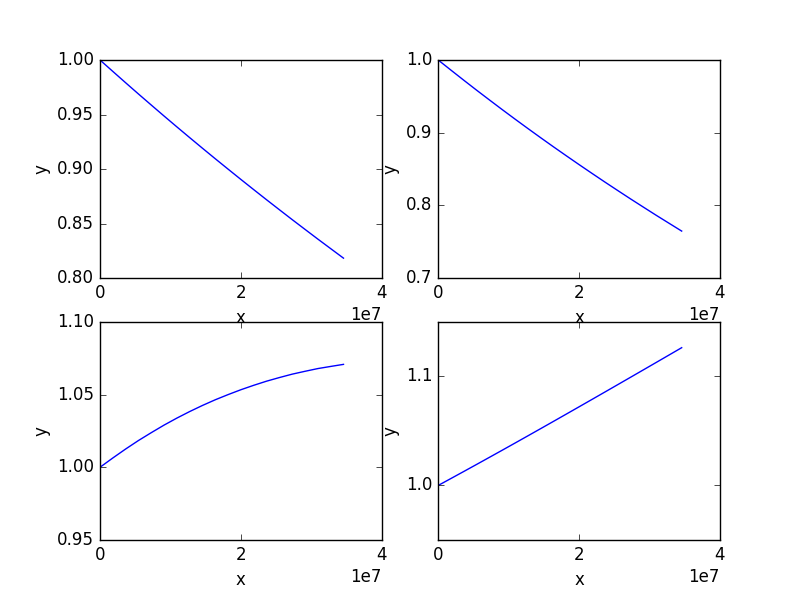
\includegraphics[scale=0.7]{../../tests/framework/user_guide/ravenTutorial/gold/subPlot/1-historyPlot_line-line-line-line.png}
  \caption{Subplot of the history for variables $A,B,C,D$.}
  \label{fig:historySubPlotLine}
\end{figure}

\section{Forward Sampling Strategies}
\label{sec:forwardSamplingStrategies}
In order to perform UQ and dynamic
probabilistic risk assessment (DPRA),
a sampling strategy needs to be employed. The sampling strategy
perturbs the input space (domain of the uncertainties) to explore
the response of a complex system in relation to selected FOMs.

The most widely used strategies to perform UQ and PRA are generally
collected in RAVEN as \textit{\textbf{Forward}} samplers. \textit{\textbf{Forward}} samplers include
all the strategies that simply perform the sampling of the input space.  These strategies sample
without exploiting, through learning approaches,
the information made available from the outcomes of evaluation previously performed (adaptive sampling) and the
common system evolution (patterns) that different sampled calculations can generate in the phase space (Dynamic Event Tree).

As mentioned in Section~\ref{susub:OverviewSamplers}, RAVEN has
several different \textit{\textbf{Forward}} samplers:
\begin{itemize}
  \item \textit{Monte-Carlo}
  \item \textit{Grid-based}
  \item \textit{Stratified} and its specialization named \textit{Latin Hyper Cube}.
\end{itemize}
In addition, RAVEN posses advanced \textit{\textbf{Forward}} sampling strategies that:
\begin{itemize}
  \item Build a grid in the input space selecting evaluation points
    based on characteristic quadratures as part of stochastic collocation
    for generalized polynomial chaos method (\textit{Sparse
    Grid Collocation} sampler);
  \item Use high-density model reduction (HDMR) a.k.a. Sobol
    decomposition to approximate a function as the sum of
    interactions with increasing complexity (\textit{Sobol} sampler).
\end{itemize}
In the following subsections, we provide examples of input files
in RAVEN using the method, with explanatory commentary.
%%%%%%%%%%%%%%%%%%%%%%%%%
%%%%%%%%  MONTE-CARLO %%%%%%%%
%%%%%%%%%%%%%%%%%%%%%%%%%
\subsection{Monte-Carlo sampling through RAVEN}
\label{sub:MCexample}
The Monte-Carlo method is one of the most-used methodologies in several mathematic disciplines. In this section,
we will explain the techniques for employing this methodology in RAVEN, and we recommend the user to read the
theory manual to explore the theory of the method.
The goals of this section are about learning how to:
 \begin{enumerate}
   \item Set up a simple Monte-Carlo sampling for perturbing the input space of a driven code
   \item Load the outputs of the code into RAVEN DataObjects (HistorySets and PointSets)
   \item Print the contents of DataObjects to file
   \item Generate plots of the sampling results.
\end{enumerate}
In order to accomplish these tasks, the following RAVEN \textbf{Entities} (XML blocks in the RAVEN input file) are needed:
\begin{enumerate}
   \item \textbf{\textit{RunInfo}}:
     \xmlExample{framework/user_guide/ForwardSamplingStrategies/forwardSamplingMontecarlo.xml}{RunInfo}
     As discussed in Section~\ref{sub:EntitiesAndFlow}, the \textit{RunInfo} \textbf{Entity} sets up the analysis
     that the user wants to perform. In this specific case, two steps (\xmlNode{Sequence}) are sequentially run
     using 12 processors (\xmlNode{batchSize}). This means that
     12 instances of the driven code are run simultaneously. Every time a simulation ends, a new one is launched.
     Note that the \xmlNode{JobName} is not required, but is useful in identifying the input file.
   \item \textbf{\textit{Files}}:
     \xmlExample{framework/user_guide/ForwardSamplingStrategies/forwardSamplingMontecarlo.xml}{Files}
     Since the driven code uses a single input file, in this section the original input is identified and
     named. As detailed in the user manual, the attribute \xmlAttr{name} represents the alias that is used in
     all the other input blocks in order to refer to this file.
   \item \textbf{\textit{Models}}:
     \xmlExample{framework/user_guide/ForwardSamplingStrategies/forwardSamplingMontecarlo.xml}{Models}
     The Model used in this example is the
     \textbf{AnalyticalBateman} external model, which is defined in section \ref{sec:analyticalbateman}.  This model uses a keyword-based input file
     and exports its output file in a CSV format, so the \textit{GenericCode} interface is used.
   \item \textbf{\textit{Distributions}}:
     \xmlExample{framework/user_guide/ForwardSamplingStrategies/forwardSamplingMontecarlo.xml}{Distributions}
     In the \xmlNode{Distributions} block, the stochastic model for the uncertainties treated by the
     \xmlNode{Sampler} is defined. In this case two distributions are defined:
     \begin{itemize}
      \item $sigma \sim \mathbb{U}(1,10)$, used to model the uncertainties
        associated with the \textit{sigma} Model variables
      \item  $decayConstant \sim \mathbb{U}(0.5e-8,1e-8)$,  used to
        model the uncertainties associated with the Model variable \textit{decay constants}.  Note that the
        same distribution can be re-used for multiple input variables, while still keeping those variables
        independent.
     \end{itemize}
   \item \textbf{\textit{Samplers}}:
     \xmlExample{framework/user_guide/ForwardSamplingStrategies/forwardSamplingMontecarlo.xml}{Samplers}
      To employ the Monte-Carlo sampling strategy ($100$ samples), a
      \xmlNode{MonteCarlo} node needs to be defined.  The
      Monte-Carlo method is employed on $eight$ model variables, each of which are listed by name
      and are associated with a distribution.
      Note that all the \textit{decay-\*} and
      \textit{sigma-\*} variables are associated with the distributions
      $decayConstant$ and $sigma$, respectively.
   \item \textbf{\textit{DataObjects}}:
     \xmlExample{framework/user_guide/ForwardSamplingStrategies/forwardSamplingMontecarlo.xml}{DataObjects}
      In this block, two \textit{DataObjects} are defined to store results: 1) a PointSet named
      ``samples'', 2) a HistorySet named ``histories''.
      Note that in the \xmlNode{Input} node all the uncertainties
      perturbed through the Monte-Carlo strategy are listed. By this, any
      realization in the input space is linked in the DataObject to the outputs listed in the
      \xmlNode{Output} node.
   \item \textbf{\textit{OutStreams}}:
     \xmlExample{framework/user_guide/ForwardSamplingStrategies/forwardSamplingMontecarlo.xml}{OutStreams}
 %%%%%%%%%%%%%%%%%%%%%%%%%%%%%%%%%%%%%%%%%%%%%%%%%%%%%%%%%%
 %figure histories
 \begin{figure}[h!]
  \centering
  \includegraphics[scale=0.7]{../../tests/framework/user_guide/ForwardSamplingStrategies/gold/RunDir/MonteCarlo/1-historyPlot_line-line-line-line.png}
  \caption{Plot of the histories generated by the Monte Carlo sampling for variables $A,B,C,D$.}
  \label{fig:historiesMCPlotLine}
 \end{figure}
 %%%%%%%%%%%%%%%%%%%%%%%%%%%%%%%%%%%%%%%%%%%%%%%%%%%%%%%%%%
 To see the results of the simulation, \xmlNode{OutStreams} are included in the input.
  In this block, both OutStream types are used:
  \begin{itemize}
    \item \textit{Print}:
     \begin{itemize}
       \item ``samples'' connected with the \textit{DataObjects} \textbf{Entity} ``samples''
                (\xmlNode{source})
       \item ``histories'' connected with the \textit{DataObjects} \textbf{Entity} ``histories'' (\xmlNode{source})
     \end{itemize}
     Note that in RAVEN, multiple entities can have the same name, as it takes a class, a type, and a name to
     uniquely identify a RAVEN object.
      When the two OutStream objects are used, all the information contained in the
      linked \textit{DataObjects} are going
    to be exported in CSV files (\xmlNode{type}).
    \item \textit{Plot}:
    \begin{itemize}
      \item ``historiesPlot'' connected with the  \textit{DataObjects}
      \textbf{Entity} ``samples''.  This plot will draw the final state of the
      variables $A,B,C,D$ with respect to the input variables $sigma$(s)
      and $decay$(s) .
      \item ``samplesPlot3D'' connected with the
      \textit{DataObjects} \textbf{Entity} ``histories''. This plot will draw the
      evolution of the variables $A,B,C,D$.
    \end{itemize}
     Note that both plots use gridded subplots. Four plots
     are placed in each of the figures.
  \end{itemize}
   \item \textbf{\textit{Steps}}:
     \xmlExample{framework/user_guide/ForwardSamplingStrategies/forwardSamplingMontecarlo.xml}{Steps}
 %%%%%%%%%%%%%%%%%%%%%%%%%%%%%%%%%%%%%%%%%%%%%%%%%%%%%%%%%%
 %figure samples
 \begin{figure}[h!]
  \centering
  \includegraphics[scale=0.7]{../../tests/framework/user_guide/ForwardSamplingStrategies/gold/RunDir/MonteCarlo/1-samplesPlot3D_scatter-scatter-scatter-scatter.png}
  \caption{Plot of the samples generated by the MC sampling for variables $A,B,C,D$.}
  \label{fig:samplesMCPlotLine}
 \end{figure}
 %%%%%%%%%%%%%%%%%%%%%%%%%%%%%%%%%%%%%%%%%%%%%%%%%%%%%%%%%%
   Once all the other entities are defined in the RAVEN input file, they must be combined in the
   \xmlNode{Steps} block, which dictates the workflow of RAVEN.  For this case,
   two \xmlNode{Steps} are defined:
   \begin{itemize}
     \item \xmlNode{MultiRun} ``sample'', used to run the multiple
     instances of the driven code and
     collect the outputs in the two \textit{DataObjects}. As it can be
     seen, the \xmlNode{Sampler} is specified to communicate to the
     \textit{Step} that the driven code needs to
     be perturbed through the Monte-Carlo sampling.
     \item  \xmlNode{IOStep} named ``writeHistories'', used to 1) dump
     the ``histories'' and ``samples'' \textit{DataObjects}
     \textbf{Entity} to a CSV file and 2) plot the data in the EPS file.
   \end{itemize}
\end{enumerate}
 Figures~\ref{fig:historiesMCPlotLine} and ~\ref{fig:samplesMCPlotLine} show the report
 generated by RAVEN of the evolution of the
 variables $A,B,C,D$ and their final values, respectively.
%%%%%%%%%%%%%%%%%%%%%%%%%
%%%%%%%%          GRID          %%%%%%%%
%%%%%%%%%%%%%%%%%%%%%%%%%
\subsection{Grid sampling through RAVEN}
\label{sub:Gridexample}
The Grid sampling method (also known as Full Factorial Design of Experiment) represents one of the simplest methodologies that can be employed in order to explore the interaction of multiple random variables with respect
selected FOMs.
The goal of this section is to show how to:
 \begin{enumerate}
   \item Set up a simple Grid sampling for performing a parametric analysis of a driven code
   \item Load the outputs of the code into the RAVEN DataObjects system
   \item Print out what contained in the DataObjects
   \item Generate basic plots of the code result.
\end{enumerate}
In order to accomplish these tasks, the following RAVEN \textbf{Entities} (XML blocks in the input files) are required:
\begin{enumerate}
   \item \textbf{\textit{RunInfo}}:
     \xmlExample{framework/user_guide/ForwardSamplingStrategies/forwardSamplingGrid.xml}{RunInfo}
   As shown in Section~\ref{sub:EntitiesAndFlow}, the \textit{RunInfo} \textbf{Entity} is intended to set up the desired analysis.
   In this specific case, two steps (\xmlNode{Sequence}) are sequentially run
   using 12 processors (\xmlNode{batchSize}). This means that
   12 instances of the driven code are  run simultaneously.
   Every time a simulation ends, a new one is launched.
   \item \textbf{\textit{Files}}:
     \xmlExample{framework/user_guide/ForwardSamplingStrategies/forwardSamplingGrid.xml}{Files}
   Since the driven code uses a single input file, in this section the original input is placed. As described in the user manual~\cite{RAVENuserManual}
   the attribute  \xmlAttr{name} represents the alias that is used in all the other input blocks in order to refer to this file.
   \item \textbf{\textit{Models}}:
     \xmlExample{framework/user_guide/ForwardSamplingStrategies/forwardSamplingGrid.xml}{Models}
 The Model here is represented by the
 \textbf{AnalyticalBateman}, which already dumps its output file in a
 CSV format (standard format that RAVEN can read). For this reason,
 the \textit{GenericCode} interface is used.
   \item \textbf{\textit{Distributions}}:
     \xmlExample{framework/user_guide/ForwardSamplingStrategies/forwardSamplingGrid.xml}{Distributions}
  In the Distributions XML section, the stochastic model for the
  uncertainties  treated by the Grid sampling are reported. In
  this case two distributions are defined:
  \begin{itemize}
    \item $sigma \sim \mathbb{U}(1,10)$, used to model the uncertainties
    associated with  the Model \textit{sigma}(s)
    \item  $decayConstant \sim \mathbb{U}(0.5e-8,1e-8)$,  used to
    model the uncertainties
    associated with  the Model \textit{decay constants}.
  \end{itemize}
   \item \textbf{\textit{Samplers}}:
     \xmlExample{framework/user_guide/ForwardSamplingStrategies/forwardSamplingGrid.xml}{Samplers}
  To employ the Grid sampling strategy, a
  \xmlNode{Grid} node needs to be specified. As shown above, in each variable section, the  \xmlNode{grid} is defined.
  The number of samples finally requested are equal to $n_{samples} = \prod_{i=1}^{n} n_{steps_{i}+1} = 256$.
  Note that, for each variable, can be defined either in probability (CDF) or in absolute value.
   \item \textbf{\textit{DataObjects}}:
     \xmlExample{framework/user_guide/ForwardSamplingStrategies/forwardSamplingGrid.xml}{DataObjects}
  Int this block, two \textit{DataObjects} are defined: 1) PointSet named
  ``samples'', and 2) HistorySet named ``histories''.
  In the \xmlNode{Input} node all the variables
  perturbed through the Grid strategy are listed. In this way, any
  realization in the input space is linked to the outputs listed in  the
  \xmlNode{Output} node.
   \item \textbf{\textit{OutStreams}}:
     \xmlExample{framework/user_guide/ForwardSamplingStrategies/forwardSamplingGrid.xml}{OutStreams}
 %%%%%%%%%%%%%%%%%%%%%%%%%%%%%%%%%%%%%%%%%%%%%%%%%%%%%%%%%%
 %figure histories
 \begin{figure}[h!]
  \centering
  \includegraphics[scale=0.7]{../../tests/framework/user_guide/ForwardSamplingStrategies/gold/RunDir/Grid/1-historyPlot_line-line-line-line.png}
  \caption{Plot of the histories generated by the Grid sampling for variables $A,B,C,D$.}
  \label{fig:historiesGridPlotLine}
 \end{figure}
 %%%%%%%%%%%%%%%%%%%%%%%%%%%%%%%%%%%%%%%%%%%%%%%%%%%%%%%%%%
  In this block, both the Out-Stream types are constructed:
  \begin{itemize}
    \item \textit{Print}:
     \begin{itemize}
       \item named ``samples'' connected with the \textit{DataObjects} \textbf{Entity} ``samples''
                (\xmlNode{source})
       \item named ``histories'' connected with the \textit{DataObjects} \textbf{Entity} ``histories'' (\xmlNode{source}).
     \end{itemize}
      When these objects get used, all the information contained in the
      linked  \textit{DataObjects} are going
    to be exported in CSV files (\xmlNode{type}).
    \item \textit{Plot}:
    \begin{itemize}
      \item named ``historiesPlot'' connected with the  \textit{DataObjects}
      \textbf{Entity} ``samples''.  This plot will draw the final state of the
      variables $A,B,C,D$ with respect to the input variables $sigma$(s)
      and $decay$(s).
      \item named ``samplesPlot3D'' connected with the
      \textit{DataObjects} \textbf{Entity} ``histories''. This plot will draw the
      evolution of the variables $A,B,C,D$.
    \end{itemize}
     As it can be noticed, both plots are of type \textit{SubPlot}. Four plots
     are placed in each of the figures.
  \end{itemize}
   \item \textbf{\textit{Steps}}:
     \xmlExample{framework/user_guide/ForwardSamplingStrategies/forwardSamplingGrid.xml}{Steps}
 %%%%%%%%%%%%%%%%%%%%%%%%%%%%%%%%%%%%%%%%%%%%%%%%%%%%%%%%%%
 %figure samples
 \begin{figure}[h!]
  \centering
  \includegraphics[scale=0.7]{../../tests/framework/user_guide/ForwardSamplingStrategies/gold/RunDir/Grid/1-samplesPlot3D_scatter-scatter-scatter-scatter.png}
  \caption{Plot of the samples generated by the Grid sampling for variables $A,B,C,D$.}
  \label{fig:samplesGridPlotLine}
 \end{figure}
 %%%%%%%%%%%%%%%%%%%%%%%%%%%%%%%%%%%%%%%%%%%%%%%%%%%%%%%%%%
   Finally, all the previously defined \textbf{Entities} can be combined in
   the \xmlNode{Steps} block. As inferable,
   two \xmlNode{Steps} have been inputted:
   \begin{itemize}
     \item \xmlNode{MultiRun} named ``sample'', is used to run the multiple
     instances of the code and
     collect the outputs in the two \textit{DataObjects}. As it can be
     seen, the \xmlNode{Sampler} is inputted to communicate to the
     \textit{Step} that the driven code needs to
     be perturbed through the Grid sampling
     \item  \xmlNode{IOStep} named ``writeHistories'', used to 1) dump
     the ``histories'' and ``samples'' \textit{DataObjects}
     \textbf{Entity} in a CSV file and 2) plot the data in the EPS file and
     on the screen.
   \end{itemize}
\end{enumerate}
 Figures~\ref{fig:historiesGridPlotLine} and ~\ref{fig:samplesGridPlotLine}  report the evolution of the
 variables $A,B,C,D$ and their final values, respectively.

%%%%%%%%%%%%%%%%%%%%%%%%%
%%%%%%%%    STRATIFIED    %%%%%%%%
%%%%%%%%%%%%%%%%%%%%%%%%%
\subsection{Stratified sampling through RAVEN}
\label{sub:Stratifiedexample}
The Stratified sampling is a class of methods that relies on the assumption that the input space (i.e.,uncertainties)
can be separated in regions (strata) based on similarity of the response of the system for input set within the
same strata. Following this assumption, the most rewarding (in terms of computational cost vs. knowledge gain)
sampling strategy would be to place one sample for each region. In this way, the same information is not
collected more than once and all the prototypical behavior are sampled at least once. In
Figure~\ref{fig:StratifiedSamplingExample}, the Stratified sampling approach is exemplified.
 \begin{figure}[h!]
  \centering
  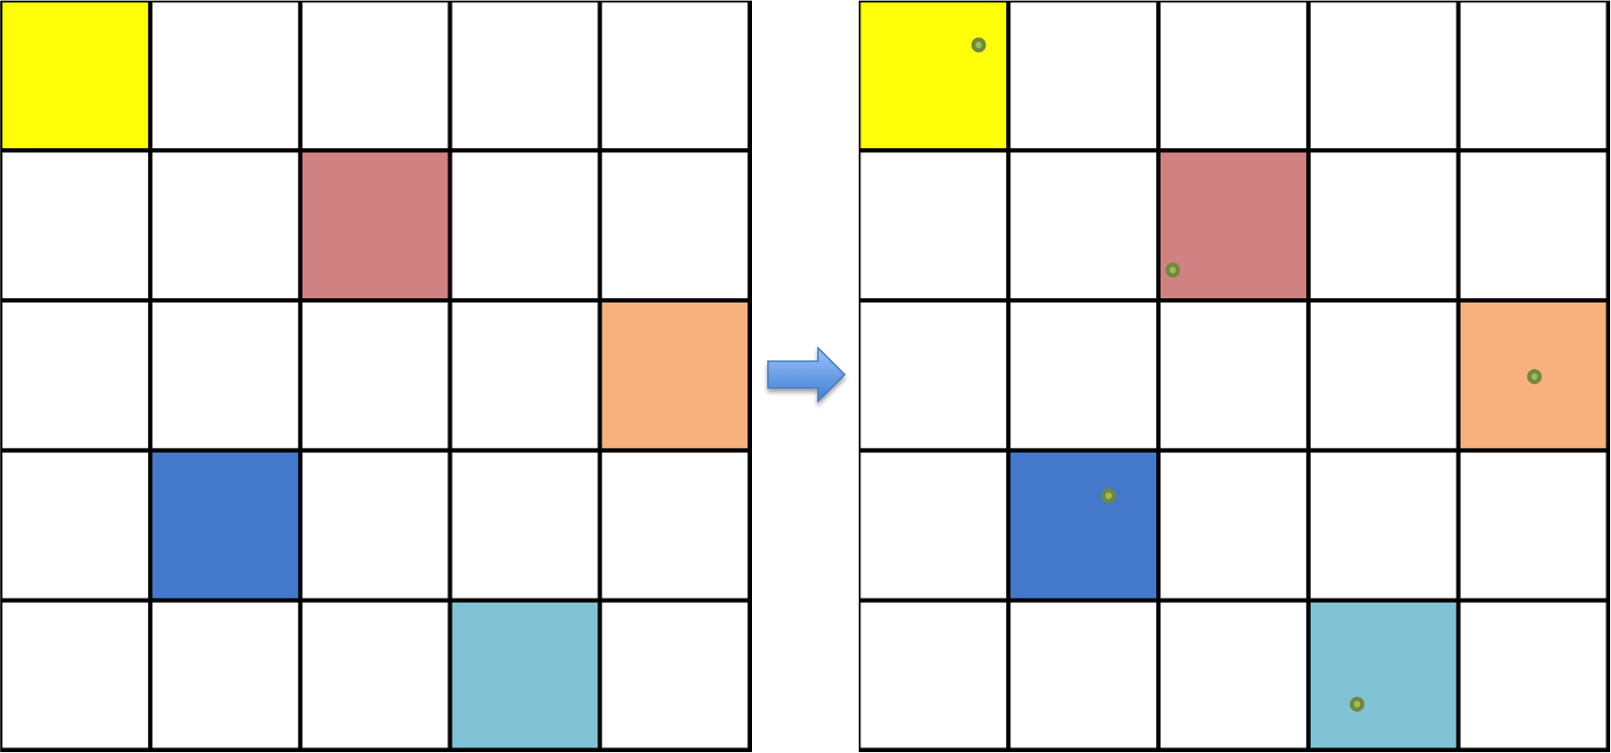
\includegraphics[scale=0.55]{pics/StratifiedSamplingExample.png}
  \caption{Example of Stratified sampling approach.}
  \label{fig:StratifiedSamplingExample}
 \end{figure}
\\The goal of this section is to show how to:
 \begin{enumerate}
   \item Set up a simple Stratified sampling in order to perform a parametric analysis on a driven code
   \item Load the outputs of the code into the RAVEN DataObjects system
   \item Print out what contained in the DataObjects
   \item Generate basic plots of the code result.
\end{enumerate}
To accomplish these tasks, the following RAVEN \textbf{Entities} (XML blocks in the input files) are defined:
\begin{enumerate}
   \item \textbf{\textit{RunInfo}}:
     \xmlExample{framework/user_guide/ForwardSamplingStrategies/forwardSamplingStratified.xml}{RunInfo}
   As reported in Section~\ref{sub:EntitiesAndFlow}, the \textit{RunInfo} \textbf{Entity} is intended to set up the analysis
   that the user wants to perform. In this specific case, two steps (\xmlNode{Sequence}) are  run
   using 12 processors (\xmlNode{batchSize}). This means that
   12 instances of the driven code are run simultaneously.
   Every time a simulation ends, a new one is launched.
   \item \textbf{\textit{Files}}:
     \xmlExample{framework/user_guide/ForwardSamplingStrategies/forwardSamplingStratified.xml}{Files}
   Since the considered code uses a single input file, in this section the original input is placed.
   The attribute  \xmlAttr{name} represents the alias that is going to be used in all the other input blocks in order to refer to this file.
   \item \textbf{\textit{Models}}:
     \xmlExample{framework/user_guide/ForwardSamplingStrategies/forwardSamplingStratified.xml}{Models}
 The Model here is represented by the
 \textbf{AnalyticalBateman}, which already dumps its output file in a
 CSV format (standard format that RAVEN can read). For this reason,
 the \textit{GenericCode} interface is used.
   \item \textbf{\textit{Distributions}}:
     \xmlExample{framework/user_guide/ForwardSamplingStrategies/forwardSamplingStratified.xml}{Distributions}
  In the Distributions XML section, the stochastic model for the
  uncertainties  treated by the Stratified sampling are reported. In
  this case two distributions are defined:
  \begin{itemize}
    \item $sigma \sim \mathbb{U}(1,10)$, used to model the uncertainties
    associated with  the Model \textit{sigma}(s)
    \item  $decayConstant \sim \mathbb{U}(0.5e-8,1e-8)$,  used to
    model the uncertainties
    associated with  the Model \textit{decay constants}.
  \end{itemize}
   \item \textbf{\textit{Samplers}}:
     \xmlExample{framework/user_guide/ForwardSamplingStrategies/forwardSamplingStratified.xml}{Samplers}
  To employ the Stratified sampling strategy, a
  \xmlNode{Stratified} node needs to be specified. In each variable section, the  \xmlNode{grid} is defined.
  It is important to mention that the number of \xmlAttr{steps} needs to be the same for each of the variables,
  since, as reported in previous section, the Stratified sampling strategy it discretizes the domain in strata.
  The number of samples finally requested is equal to $n_{samples} = n_{steps} = 100$.
  If the grid for each variables is defined in CDF and of  \xmlAttr{type} = ``equal'', the Stratified
  sampling corresponds to the well-known Latin Hyper Cube sampling.
   \item \textbf{\textit{DataObjects}}:
     \xmlExample{framework/user_guide/ForwardSamplingStrategies/forwardSamplingStratified.xml}{DataObjects}
  In this block, two \textit{DataObjects} are defined: 1) PointSet named
  ``samples'', 2) HistorySet named ``histories''.
  In the \xmlNode{Input} node all the variables
  perturbed through the Stratified strategy are listed. In this way, any
  realization in the input space is linked to the outputs listed in  the
  \xmlNode{Output} node.
   \item \textbf{\textit{OutStreams}}:
     \xmlExample{framework/user_guide/ForwardSamplingStrategies/forwardSamplingStratified.xml}{OutStreams}
 %%%%%%%%%%%%%%%%%%%%%%%%%%%%%%%%%%%%%%%%%%%%%%%%%%%%%%%%%%
 %figure histories
 \begin{figure}[h!]
  \centering
  \includegraphics[scale=0.7]{../../tests/framework/user_guide/ForwardSamplingStrategies/gold/RunDir/Stratified/1-historyPlot_line-line-line-line.png}
  \caption{Plot of the histories generated by the Stratified sampling for variables $A,B,C,D$.}
  \label{fig:historiesStratifiedPlotLine}
 \end{figure}
 %%%%%%%%%%%%%%%%%%%%%%%%%%%%%%%%%%%%%%%%%%%%%%%%%%%%%%%%%%
  In this block, both the Out-Stream types are constructed:
  \begin{itemize}
    \item \textit{Print}:
     \begin{itemize}
       \item named ``samples'' connected with the \textit{DataObjects} \textbf{Entity} ``samples''
                (\xmlNode{source})
       \item named ``histories'' connected with the \textit{DataObjects} \textbf{Entity} ``histories'' (\xmlNode{source}).
     \end{itemize}
      When these objects get used, all the information contained in the
      linked  \textit{DataObjects} are going
    to be exported in CSV files (\xmlNode{type}).
    \item \textit{Plot}:
    \begin{itemize}
      \item named ``historiesPlot'' connected with the  \textit{DataObjects}
      \textbf{Entity} ``samples''.  This plot will draw the final state of the
      variables $A,B,C,D$ with respect to the input variables $sigma$(s)
      and $decay$(s)
      \item named ``samplesPlot3D'' connected with the
      \textit{DataObjects} \textbf{Entity} ``histories''. This plot will draw the
      evolution of the variables $A,B,C,D$.
    \end{itemize}
     As it can be noticed, both plots are of type \textit{SubPlot}. Four plots
     are going to be placed in each of the figures.
  \end{itemize}
   \item \textbf{\textit{Steps}}:
     \xmlExample{framework/user_guide/ForwardSamplingStrategies/forwardSamplingStratified.xml}{Steps}
 %%%%%%%%%%%%%%%%%%%%%%%%%%%%%%%%%%%%%%%%%%%%%%%%%%%%%%%%%%
 %figure samples
 \begin{figure}[h!]
  \centering
  \includegraphics[scale=0.7]{../../tests/framework/user_guide/ForwardSamplingStrategies/gold/RunDir/Stratified/1-samplesPlot3D_scatter-scatter-scatter-scatter.png}
  \caption{Plot of the samples generated by the Stratified sampling for variables $A,B,C,D$.}
  \label{fig:samplesStratifiedPlotLine}
 \end{figure}
 %%%%%%%%%%%%%%%%%%%%%%%%%%%%%%%%%%%%%%%%%%%%%%%%%%%%%%%%%%
   Finally, all the previously defined \textbf{Entities} can be combined in
   the \xmlNode{Steps} block. As inferable,
   two \xmlNode{Steps} have been inputted:
   \begin{itemize}
     \item \xmlNode{MultiRun} named ``sample'', used to run the multiple
     instances of the driven code and
     collect the outputs in the two \textit{DataObjects}. As it can be
     seen, the \xmlNode{Sampler} is inputted to communicate to the
     \textit{Step} that the driven code needs to
     be perturbed through the Stratified sampling.
     \item  \xmlNode{IOStep} named ``writeHistories'', used to 1) dump
     the ``histories'' and ``samples'' \textit{DataObjects}
     \textbf{Entity} in a CSV file and 2) plot the data in the EPS file and
     on the screen.
   \end{itemize}
\end{enumerate}
 As previously mentioned, Figures~\ref{fig:historiesStratifiedPlotLine} and ~\ref{fig:samplesStratifiedPlotLine}  report the evolution of the
 variables $A,B,C,D$ and their final values, respectively.

%%%%%%%%%%%%%%%%%%%%%%%%%

\subsection{Sparse Grid Collocation sampling through RAVEN}
\label{sub:SGcsamplingExample}
The Sparse Grid Collocation sampler represents an advanced methodology to perform Uncertainty Quantification. They aim
to explore the input space leveraging the information contained in the associated probability density functions. It builds on generic Grid sampling by selecting evaluation points based on characteristic quadratures as part of stochastic collocation for generalized polynomial chaos uncertainty quantification. In collocation an N-D grid is constructed, with each uncertain variable providing an axis. Along each axis, the points of evaluation correspond to quadrature points necessary to integrate polynomials. In the simplest (and most naive) case, a N-D tensor product of all possible combinations of points from each dimension’s quadrature is constructed as sampling points. The number of necessary samples can be reduced by employing Smolyak-like sparse grid algorithms, which use reduced combinations of polynomial orders to reduce the necessary sampling space.
\\The goals of this section are about learning how to:
 \begin{enumerate}
   \item Set up a Sparse Grid Collocation sampling for the construction of a suitable surrogate model of a driven code
   \item Construct a GaussPolynomialRom surrogate model (training stage)
   \item Use the constructed GaussPolynomialRom surrogate model instead of the driven code.
\end{enumerate}
To accomplish these tasks, the following RAVEN \textbf{Entities} (XML blocks in the input files) need to be defined:
\begin{enumerate}
   \item \textbf{\textit{RunInfo}}:
     \xmlExample{framework/user_guide/ForwardSamplingStrategies/forwardSamplingSparseGrid.xml}{RunInfo}
   As reported in section~\ref{sub:EntitiesAndFlow}, the \textit{RunInfo} \textbf{Entity} is intended to set up the analysis
   that the user wants to perform. In this specific case, six steps (\xmlNode{Sequence}) are going to be sequentially run
   using twelve processors (\xmlNode{batchSize}).  The first two steps build the ROM
   (\xmlString{sample}, \xmlString{train}), the next two validate
   the ROM against the original Code Model (\xmlString{validateModel}, \xmlString{validateROM}),
   and the last two produce plots and print data (\xmlString{output\_print}, \xmlString{output\_plot}).
   \item \textbf{\textit{Files}}:
     \xmlExample{framework/user_guide/ForwardSamplingStrategies/forwardSamplingSparseGrid.xml}{Files}
   Since the driven code uses a single input file, in this section the original input is placed. As detailed in the user manual
   the attribute  \xmlAttr{name} represents the alias that is going to be used in all the other input blocks in order to refer to this file.
   \item \textbf{\textit{Models}}:
     \xmlExample{framework/user_guide/ForwardSamplingStrategies/forwardSamplingSparseGrid.xml}{Models}
 The goal of this example is the generation of a \text{GaussPolynomialRom}
 for subsequent usage instead of the original code.  In addition to the previously explained Code model,
 the ROM of type \textit{GaussPolynomialRom} is specified here. The ROM is generated through a Sparse Grid
 Collocation sampling strategy. All 4 targets $A,B,C,D$ are modeled through this ROM as function
 of the uncertain $sigma$ and $decay$ parameters.  Note that the \xmlNode{Interpolation} nodes are not
 required, but are included for the sake of demonstration.
   \item \textbf{\textit{Distributions}}:
     \xmlExample{framework/user_guide/ForwardSamplingStrategies/forwardSamplingSparseGrid.xml}{Distributions}
  In the Distributions XML section, the stochastic model for the
  uncertainties  treated by the Sparse Grid Collocation sampling are reported. In
  this case eight distributions are defined:
  \begin{itemize}
    \item $sigmaA \sim \mathbb{U}(6.9,8.1)$, used to model the uncertainty
    associated with  the Model \textit{sigma-A}
    \item $sigmaB \sim \mathbb{U}(3.9,5.1)$, used to model the uncertainty
    associated with  the Model \textit{sigma-B}
    \item $sigmaC \sim \mathbb{U}(1.9,3.1)$, used to model the uncertainty
    associated with  the Model \textit{sigma-C}
    \item $sigmaD \sim \mathbb{U}(0.9,1.1)$, used to model the uncertainty
    associated with  the Model \textit{sigma-D}
    \item  $decayConstantA \sim \mathbb{U}(3.8e-9,5.2e-9)$,  used to
    model the uncertainty
    associated with  the Model \textit{decay-A}
    \item  $decayConstantB \sim \mathbb{U}(5.8e-9,7.2e-9)$,  used to
    model the uncertainty
    associated with  the Model \textit{decay-B}
    \item  $decayConstantC \sim \mathbb{U}(6.8e-9,8.2e-9)$,  used to
    model the uncertainty
    associated with  the Model \textit{decay-C}
    \item  $decayConstantD \sim \mathbb{U}(7.8e-9,9.2e-9)$,  used to
    model the uncertainty
    associated with  the Model \textit{decay-D}.
  \end{itemize}
   \item \textbf{\textit{Samplers}}:
     \xmlExample[rom,ROM,SparseGridCollocation,MonteCarlo]{framework/user_guide/ForwardSamplingStrategies/forwardSamplingSparseGrid.xml}{Samplers}
  In order to employ the Sparse Grid Collocation sampling strategy, a
  \xmlNode{SparseGridCollocation} node needs to be defined.
  As can be
  seen from above, each variable is associated with a different distribution,
  defined in the  \xmlNode{Distributions} block.
  In addition, the \textit{GaussPolynomialRom} \xmlNode{ROM} is linked to the \xmlNode{SparseGridCollocation}
  sampler.  Because this sampler is used exclusively to build the ROM, some of the parameters of the ROM are
  needed by the sampler, and this connection makes that communication possible.  The setting of this ROM
  (e.g. polynomial order, Index set method, etc.) determines how the Stochastic Collocation Method is
  employed.

  Additionally, a \xmlNode{MonteCarlo} sampler is set up for validating the ROM against the original Code.  The random
  number generation seed (\xmlNode{initialSeed}) is specified and set to reset on each use
  (\xmlNode{reseedEachIteration}) so that the Monte Carlo sampler can be used to compare the ROM against the
  original model.  We use twenty samples (\xmlNode{limit}) to sample the ROM and the model, and then print and
  plot both data sets to compare them.
   \item \textbf{\textit{DataObjects}}:
     \xmlExample[rom,SparseGridCollocation]{framework/user_guide/ForwardSamplingStrategies/forwardSamplingSparseGrid.xml}{DataObjects}
  In this block, four \textit{DataObjects} are defined:
  1) a PointSet named ``inputPlaceholder'' used as a placeholder input for the ROM sampling step,
  2) a HistorySet named ``histories'' used to collect the samples needed to train the ROM,
  3) a PointSet named ``samplesModel'' to store the Code responses from Monte Carlo samples, and
  4) a PointSet named ``samplesROM'' to store the ROM responses from Monte Carlo samples.
 %%%%%%%%%%%%%%%%%%%%%%%%%%%%%%%%%%%%%%%%%%%%%%%%%%%%%%%%%%
 %%%%%%%%%%%%%%%%%%%%%%%%%%%%%%%%%%%%%%%%%%%%%%%%%%%%%%%%%%
 %figure histories
 \begin{figure}[h!]
  \centering
  \includegraphics[scale=0.7]{../../tests/framework/user_guide/ForwardSamplingStrategies/gold/RunDir/SparseGrid/1-historyPlot_line-line-line-line.png}
  \caption{Plot of the training samples generated by the SparseGridCollocation sampling for variables $A,B,C,D$.}
  \label{fig:historiesSparseGridPlotLine}
 \end{figure}
 %%%%%%%%%%%%%%%%%%%%%%%%%%%%%%%%%%%%%%%%%%%%%%%%%%%%%%%%%%
 %%%%%%%%%%%%%%%%%%%%%%%%%%%%%%%%%%%%%%%%%%%%%%%%%%%%%%%%%%
   \item \textbf{\textit{OutStreams}}:
     \xmlExample{framework/user_guide/ForwardSamplingStrategies/forwardSamplingSparseGrid.xml}{OutStreams}
  In this block, the following Out-Stream types are constructed:
  \begin{itemize}
    \item \textit{Print}:
     \begin{itemize}
       \item named ``samplesModel'' connected with the \textit{DataObjects} \textbf{Entity} ``samplesModel''
                (\xmlNode{source})
       \item named ``samplesROM'' connected with the \textit{DataObjects} \textbf{Entity} ``samplesROM''
                (\xmlNode{source})
       \item named ``histories'' connected with the \textit{DataObjects} \textbf{Entity} ``histories'' (\xmlNode{source})
       \item named ``rom\_output'' connected with the \textit{ROM} \textbf{Entity} ``rom'' (\xmlNode{source}).
     \end{itemize}
      When these objects get used, all the information contained in the
      linked  \textit{DataObjects} are going
    to be exported in ether CSV files for DataObjects or XML files for ROMs (\xmlNode{type}).
    \item \textit{Plot}:
    \begin{itemize}
      \item named ``historyPlot'' connected with the  \textit{DataObjects}
      \textbf{Entity} ``histories''.  This plot will draw the time-dependent state of the
      variables $A,B,C,D$ with respect to the input variables $sigma$(s)
      and $decay$(s)
      \item named ``samplesModelPlot3D'' connected with the
      \textit{DataObjects} \textbf{Entity} ``samplesModel''. This plot will draw the
      variables $A,B,C,D$ as Monte Carlo sampled on the Code.
      \item named ``samplesROMPlot3D'' connected with the
      \textit{DataObjects} \textbf{Entity} ``samplesROM''. This plot will draw the
      variables $A,B,C,D$ as Monte Carlo sampled on the ROM.
    \end{itemize}
     As it can be noticed, both plots are of type \textit{SubPlot}. Four plots
     are going to be placed in each of the figures.
  \end{itemize}
   \item \textbf{\textit{Steps}}:
     \xmlExample[rom,SparseGridCollocation]{framework/user_guide/ForwardSamplingStrategies/forwardSamplingSparseGrid.xml}{Steps}
  %%%%%%%%%%%%%%%%%%%%%%%%%%%%%%%%%%%%%%%%%%%%%%%%%%%%%%%%%%
 %figure samples
 \begin{figure}[h!]
  \centering
  \includegraphics[scale=0.7]{../../tests/framework/user_guide/ForwardSamplingStrategies/gold/RunDir/SparseGrid/1-samplesModelPlot3D_scatter-scatter-scatter-scatter.png}
  \caption{Plot of validation samples generated by Monte Carlo sampling on the Code for variables $A,B,C,D$.}
  \label{fig:samplesSparseGridPlotModel}
 \end{figure}
 %%%%%%%%%%%%%%%%%%%%%%%%%%%%%%%%%%%%%%%%%%%%%%%%%%%%%%%%%%
   Finally, the previously defined \textbf{Entities} can be combined in
   the \xmlNode{Steps} block.
   The following \xmlNode{Steps} have been defined:
   \begin{itemize}
     \item \xmlNode{MultiRun} named ``sample'', used to run the training
     samples of the driven code and
     collect the outputs in the \textit{DataObjects}.
     The \xmlNode{Sampler} is specified to communicate to the
     \textit{Step} that the driven code needs to
     be sampled through the Sparse Grid Collocation sampling strategy;
     \item \xmlNode{RomTrainer} named ``train'', used to train (i.e.,
     construct) the GaussPolynomial ROM. This step is essential if the
     user want to use the ROM in later steps;
     \item \xmlNode{MultiRun} named ``sampleModel'', used to run the
     Monte Carlo perturbed samples of the original Model for use in verification.  The results are
     collected in the \textit{samplesModel} \textit{DataObjects}.
     \item \xmlNode{MultiRun} named ``sampleROM'', used to run the
     Monte Carlo perturbed samples of the previously constructed ROM for use in verificaiton.  The results are
     collected in the \textit{samplesROM} \textit{DataObjects}.
     \item  \xmlNode{IOStep} named ``output\_print'', used to dump
     the ``histories'', ``samplesModel'' and ``samplesROM'' \textit{DataObjects}
     \textbf{Entity} in a CSV file,
     \item  \xmlNode{IOStep} named ``output\_plot'', used to
     plot the data and store it in the PNG file and
     on the screen.
   \end{itemize}
\end{enumerate}
 As previously mentioned, Figure~\ref{fig:historiesSparseGridPlotLine}
 shows the evolution of the outputs $A,B,C,D$ under uncertainties.
 Figures~\ref{fig:samplesSparseGridPlotModel} and
 \ref{fig:samplesROMSparseGridPlotROM} show the final responses
 of the sampling employed using the driven code and the ROM,
 respectively. As it can be seen, the constructed ROM can accurately
 represent the response of the driven code. This example shows the
 potential of reduced order modeling, in general, and of the
 \textit{GaussPolynomialRom}, in particular.

  %%%%%%%%%%%%%%%%%%%%%%%%%%%%%%%%%%%%%%%%%%%%%%%%%%%%%%%%%%
 %figure samples
 \begin{figure}[h!]
  \centering
  \includegraphics[scale=0.7]{../../tests/framework/user_guide/ForwardSamplingStrategies/gold/RunDir/SparseGrid/1-samplesROMPlot3D_scatter-scatter-scatter-scatter.png}
  \caption{Plot of validation samples generated by Monte Carlo sampling on the ROM for variables $A,B,C,D$.}
  \label{fig:samplesROMSparseGridPlot}
 \end{figure}
 %%%%%%%%%%%%%%%%%%%%%%%%%%%%%%%%%%%%%%%%%%%%%%%%%%%%%%%%%%









\section{Adaptive Sampling Strategies}
\label{sec:adaptiveSamplingStrategies}
Performing UQ and Dynamic PRA can be
challenging from a computational point of view. The \textit{Forward}
sampling strategies reported in the previous Section can lead to a large number of
unnecessary evaluations of the physical model leading to an unacceptable resource expenses (CPU time).
In addition, the \textit{Forward} methodologies are not designed to leverage the information
content that is extractable from the simulations already concluded.

To overcome these limitations, in RAVEN several adaptive algorithms are available:
\begin{enumerate}
  \item \textit{Limit Surface Search}
  \item \textit{Adaptive Dynamic Event Tree}
  \item \textit{Adaptive Hybrid Dynamic Event Tree}
  \item \textit{Adaptive Sparse Grid}
  \item \textit{Adaptive Sobol Decomposition}.
\end{enumerate}
In this Section, we will only show how to use the first algorithm.

%%%%%%%%%%%%%%%%
\subsection{Limit Surface Search sampling through RAVEN}
\label{sub:LSsamplingExample}
The goal of this Section is to learn how to:
 \begin{enumerate}
   \item Set up a LS Search sampling for efficiently perturb a driven code
   \item Use the LS Integral Post-processor for computing the probability of failure of the system subject to the same
   ``goal'' function
   \item Plot the obtained LS.
\end{enumerate}
In order to accomplish these tasks, the following RAVEN \textbf{Entities} (XML blocks in the input files) are defined:
\begin{enumerate}
   \item \textbf{\textit{RunInfo}}:
     \xmlExample[arg,extension,pauseAtEnd,overwrite]{framework/user_guide/AdaptiveSamplingStrategies/adaptiveSamplingLSsearch.xml}{RunInfo}
   As shown in Section~\ref{sub:EntitiesAndFlow}, the \textit{RunInfo} \textbf{Entity} is intended to set up the analysis
   that the user wants to perform. In this specific case, three steps (\xmlNode{Sequence}) are  sequentially run
   using eight processors (\xmlNode{batchSize}).
   \item \textbf{\textit{Files}}:
     \xmlExample[arg,extension,pauseAtEnd,overwrite]{framework/user_guide/AdaptiveSamplingStrategies/adaptiveSamplingLSsearch.xml}{Files}
   Since the driven code uses a single input file, in this Section the original input is placed. As detailed in the user manual
   the attribute  \xmlAttr{name} represents the alias that is going to be
   used in all the other input blocks in order to refer to this file.
   \\In addition the output file used in \xmlNode{Sequence}
   \textit{computeLSintegral} is here inputted.
   \item \textbf{\textit{Models}}:
     \xmlExample[arg,extension,pauseAtEnd,overwrite]{framework/user_guide/AdaptiveSamplingStrategies/adaptiveSamplingLSsearch.xml}{Models}
 As mentioned above, the goal of this example is the employment of
 an efficient sampling strategy, having as goal the determination of the
 failure of a system.

 In addition to the previously explained Code
 model,
 the ROM of type \textit{SciKitLearn} is here specified. The ROM will be
 used in the adaptive sampling strategy \textit{LimitSurfaceSearch} in
 order to accelerate the convergence of the method. As it can be seen,
 a nearest neighbor classifier is used, targeting only two uncertainties
 $sigma-A and decay-A$.
 \\ For the computation of the probability of failure (see the following), a
 Post-Processor (PP) of type \textit{LimitSurfaceIntegral} is here
 specified.This PP performs an integral of the LS
 generated by the adaptive sampling technique.
   \item \textbf{\textit{Distributions}}:
     \xmlExample{framework/user_guide/AdaptiveSamplingStrategies/adaptiveSamplingLSsearch.xml}{Distributions}
  In the Distributions XML Section, the stochastic model for the
  uncertainties  treated by the LS search sampling are reported. In
  this case two distributions are defined:
  \begin{itemize}
    \item $sigmaA \sim \mathbb{U}(0,1000)$, used to model the uncertainty
    associated with  the Model \textit{sigma-A}
    \item  $decayConstantA \sim \mathbb{U}(1e-8,1e-7)$,  used to
    model the uncertainty
    associated with  the Model \textit{decay-A}.
  \end{itemize}
   \item \textbf{\textit{Samplers}}:
     \xmlExample[arg,extension,pauseAtEnd,overwrite]{framework/user_guide/AdaptiveSamplingStrategies/adaptiveSamplingLSsearch.xml}{Samplers}
  In order to employ the LS search sampling strategy, a
  \xmlNode{LimitSurfaceSearch} node needs to be inputted.
  As it can be
  seen from above, each variable is associated to a different distribution
  defined in the  \xmlNode{Distributions} block.
  In addition, the \textit{AccelerationROM}  \xmlNode{ROM} is inputted.
  As already mentioned, this ROM (of type classifier) is used to
  accelerate the convergence of the LS Search method.
  In addition, the goal function \textit{goalFunction}  and the
  \textit{samples} are here reported.
  \\For this example, a convergence criterion of $1.0e-5$ is set. To reach such a confidence with a Monte-Carlo, millions of
  samples would be needed.
   \item \textbf{\textit{Functions}}:
     \xmlExample[arg,extension,pauseAtEnd,overwrite]{framework/user_guide/AdaptiveSamplingStrategies/adaptiveSamplingLSsearch.xml}{Functions}
 As already mentioned, the LS search sampling strategy uses
 a goal function in order to identify the regions of the uncertain space
 that are more informative. The \textit{goalFunction} used for this
 example is reported below. As it can be seen, if the final response $A$
 is $<=$ of $0.3$ , the system is considered to be in a ``safe'' condition.
\begin{lstlisting}[language=python]
def __residuumSign(self):
  returnValue = 1.0
  if self.A  <= 0.3:
    returnValue = -1.0
  return returnValue
\end{lstlisting}

   \item \textbf{\textit{DataObjects}}:
     \xmlExample[arg,extension,pauseAtEnd,overwrite]{framework/user_guide/AdaptiveSamplingStrategies/adaptiveSamplingLSsearch.xml}{DataObjects}
      In this block, three \textit{DataObjects} are defined: 1) PointSet
      named ``samples'' used to collect the final outcomes of the code, 2)
      HistorySet named ``histories'' in which the full time responses of the
      variables $A,B,C,D$ are going to be stored, 3) PointSet named
      ``limitSurface'' used  to export the LS location (in the uncertain space) during the employment of the sampling strategy.
   \item \textbf{\textit{OutStreams}}:
     \xmlExample[arg,extension,pauseAtEnd,overwrite]{framework/user_guide/AdaptiveSamplingStrategies/adaptiveSamplingLSsearch.xml}{OutStreams}
     Several out streams are included in this workflow, two for printing and three for plotting:
     \begin{itemize}
       \item ``samples'', which writes the validation sample contents of the \xmlString{samples} PointSet DataObject to a CSV file,
       \item ``histories'', which writes the sampling contents of the \xmlString{histories} HistorySet DataObject to a
         set of connected CSV files,
       \item ``historyPlot'', which plots the evolution of the samples taken,
       \item ``limitSurfacePlot'', which plots the limit surface discovered by the PostProcessor,
       \item ``samplesPlot3D'', which plots the final state of the samples taken against the figures of merit.
     \end{itemize}
     The plots demonstrate how visualization of three-dimensional data, time-dependent data, and limit
     surfaces can be realized using RAVEN.
 %%%%%%%%%%%%%%%%%%%%%%%%%%%%%%%%%%%%%%%%%%%%%%%%%%%%%%%%%%
 %%%%%%%%%%%%%%%%%%%%%%%%%%%%%%%%%%%%%%%%%%%%%%%%%%%%%%%%%%
 %figure samples
 \begin{figure}[h!]
  \centering
  \includegraphics[scale=0.7]{../../tests/framework/user_guide/AdaptiveSamplingStrategies/gold/LSsearch/1-samplesPlot3D_scatter-scatter.png}
  \caption{Plot of the samples generated by the LS search sampling for variables $A,B$.}
  \label{fig:LS_pointsets}
 \end{figure}
 %%%%%%%%%%%%%%%%%%%%%%%%%%%%%%%%%%%%%%%%%%%%%%%%%%%%%%%%%%
 %%%%%%%%%%%%%%%%%%%%%%%%%%%%%%%%%%%%%%%%%%%%%%%%%%%%%%%%%%
   \item \textbf{\textit{Steps}}:
     \xmlExample[arg,extension,pauseAtEnd,overwrite]{framework/user_guide/AdaptiveSamplingStrategies/adaptiveSamplingLSsearch.xml}{Steps}
  %%%%%%%%%%%%%%%%%%%%%%%%%%%%%%%%%%%%%%%%%%%%%%%%%%%%%%%%%%
 %figure samples
 \begin{figure}[h!]
  \centering
  \includegraphics[scale=0.7]{../../tests/framework/user_guide/AdaptiveSamplingStrategies/gold/LSsearch/1-historyPlot_line-line-line-line.png}
  \caption{Plot of the histories generated by the LS search method for variables $A,B,C,D$.}
  \label{fig:LS_histories}
 \end{figure}
 %%%%%%%%%%%%%%%%%%%%%%%%%%%%%%%%%%%%%%%%%%%%%%%%%%%%%%%%%%
   Finally, all the previously defined \textbf{Entities} can be combined in
   the \xmlNode{Steps} block. As inferable,
   three \xmlNode{Steps} have been inputted:
   \begin{itemize}
     \item \xmlNode{MultiRun} named ``sample'', used to run the multiple
     instances of the driven code and
     collect the outputs in the two \textit{DataObjects}. As it can be
     seen, the \xmlNode{Sampler} is inputted to communicate to the
     \textit{Step} that the driven code needs to
     be perturbed through the LS search sampling strategy;
     \item \xmlNode{PostProcess} named ``computeLSintegral'', used to
     compute the probability of failure of the system based on the LS generated employing the LS search strategy. This
     probability is computed integrating the LS with a Monte-Carlo
     method.
     \item  \xmlNode{IOStep} named ``writeHistories'', used to 1) export
     the ``histories'' and ``samples''  \textit{DataObjects}
     \textbf{Entity} in a CSV file and 2) plot the data and the Limit Surface
     in  PNG files and on the screen.
   \end{itemize}
\end{enumerate}
 Figure~\ref{fig:LS_histories}
 shows the evolution of the outputs $A,B,C,D$ under uncertainties.
 Figure~\ref{fig:LS_pointsets} shows the final responses  of $A and B$
 of the sampling employed using the driven code.
 Figure~\ref{fig:LSplot}  shows the limit surface for this particular
 example. Only $367$ samples were needed in order to reach the full
 convergence.
 \\The integration of the LS determines a probability of failure of
 $~3.45e-2$.
  %%%%%%%%%%%%%%%%%%%%%%%%%%%%%%%%%%%%%%%%%%%%%%%%%%%%%%%%%%
 %figure samples
 \begin{figure}[h!]
  \centering
  \includegraphics[scale=0.7]{../../tests/framework/user_guide/AdaptiveSamplingStrategies/gold/LSsearch/1-limitSurfacePlot_scatter.png}
  \caption{Limit Surface generated by the LS search method.}
  \label{fig:LSplot}
 \end{figure}
 %%%%%%%%%%%%%%%%%%%%%%%%%%%%%%%%%%%%%%%%%%%%%%%%%%%%%%%%%%









\input{restartSampling.tex}
\section{Reduced Order Modeling through RAVEN}
\label{sec:ROMraven}
The development of high-fidelity codes, for thermal-hydraulic systems
and integrated multi-physics, has undergone a significant acceleration
in the last years. Multi-physics codes simulate
multiple physical models or multiple simultaneous physical phenomena,
in a integrated solving environment. Multi-physics typically
solves coupled systems of partial differential equations, generally
characterized by several different geometrical and time scales.

The new multi-physics codes are characterized by remarkable
improvements
in the approximation of physics (high approximation order and reduced
use of empirical correlations). This greater fidelity is generally
accompanied by a greater computational effort (calculation time
increased). This peculiarity is an
obstacle in the application of  computational techniques of
quantification of uncertainty and risk associated with the operation of
particular industrial plant (e.g., a nuclear reactor).

A solution to this problem is represented by the
usage
of highly effective sampling strategies. Sometimes also these
approaches is not enough
in order to perform a comprehensive UQ and PRA analysis. In these
cases the help of reduced order modeling is essential.

RAVEN has support of several different ROMs,
such as:
\begin{enumerate}
  \item \textit{Nearest Neighbors approaches}
  \item \textit{Support Vector Machines}
  \item \textit{Inverse Weight regressors}
  \item \textit{Spline regressors }, etc.
\end{enumerate}

A ROM, also known a surrogate
model, is a mathematical representation of a system, used to predict
a FOM of a physical system.

The ``training'' is a process of setting the internal parameters of the ROM from a set
of samples generated the physical model, .e.,
 the high-fidelity simulator (RELAP-7, RELAP5
3D, PHISICS, etc.),
\begin{figure}[h!]
  \centering
  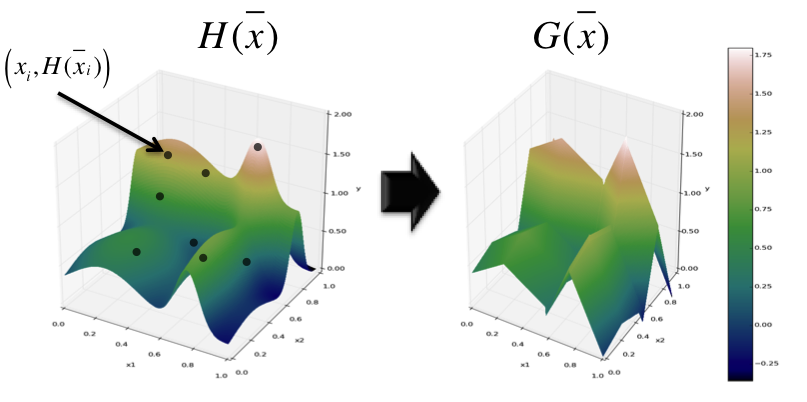
\includegraphics[width=1.0\textwidth]  {pics/ROMexampleOfPhysicalSystem.png}
  \caption{Example of reduced order model representation of physical system (regression).}
  \label{fig:ROMexampleOfPhysicalSystem}
\end{figure}

Two characteristics of these models
are generally assumed (even if exceptions are possible):
\begin{enumerate}
  \item The higher the number of realizations in the training sets, the
higher is the accuracy of the prediction performed by the ROM is. This
statement is true for most of the cases, although some ROMs might be
subject to the over-fitting issues. The over-fitting phenomenon is not
analyzed in this thesis, since its occurrence highly depends on the
algorithm type, and, hence, the problem needs to be analyzed for all
the large number of ROM types available;
  \item The smaller the size of the input (uncertain) domain with
  respect to the variability of the system response, the more likely the
  ROM is able to represent the system response space.
\end{enumerate}

The goals of this section are about learning how to:
 \begin{enumerate}
   \item Set up a sampling strategy to construct multiple ROMs, perturbing a driven code
   \item Train the different ROMs with the data-set obtained by the applied sampling strategy;
   \item Use the same sampling strategy, perturbing the ROMs
   \item Plot the responses of the driven code and ROMs, respectively.
\end{enumerate}
In order to accomplish these tasks, the following RAVEN \textbf{Entities} (XML blocks in the input files) need to be defined:
\begin{enumerate}
   \item \textbf{\textit{RunInfo}}:
     \xmlExample{framework/user_guide/ReducedOrderModeling/reducedOrderModeling.xml}{RunInfo}
   As in the other examples, the the \textit{RunInfo} \textbf{Entity} is intended  to set up the analysis sequence that
   needs to be performed. In this specific case, eight steps  (\xmlNode{Sequence}) are going to be sequentially run
   using eight processors (\xmlNode{batchSize}).
   \\In the first step, the original physical model is going to be sampled. The obtained results are going to be used to
   train three different ROMs.These ROMs are sampled by the same strategy used in the first step in order to compare the
   ROMs' responses with the ones coming from the original physical model.
   \item \textbf{\textit{Files}}:
     \xmlExample{framework/user_guide/ReducedOrderModeling/reducedOrderModeling.xml}{Files}
   Since the driven code uses a single input file, the original input is placed in this section. As detailed in the user manual
   the attribute  \xmlAttr{name} represents the alias that is going to be
   used in all the other input blocks in order to refer to this file.
   \item \textbf{\textit{Models}}:
     \xmlExample{framework/user_guide/ReducedOrderModeling/reducedOrderModeling.xml}{Models}
 As mentioned above, the goal of this example is the employment of
 a sampling strategy in order to construct multiple types of ROMs.
 \\Indeed, in addition to the previously explained Code
 model,
 three different ROMs (GP, SVM and IDW) are here specified. The ROMs will be
 constructed (``trained'') through the data-set generated by the sampling of the physical model. Once trained, they are going
 to be used in place of the original physical model.
 \\As it can be seen,
 the ROMs will be constructed considering four features ($sigma-A,\,sigma-B,\, decay-A \,,and \, decay-B$) and two targets
 ($A \, and \, B$).
   \item \textbf{\textit{Distributions}}:
     \xmlExample{framework/user_guide/ReducedOrderModeling/reducedOrderModeling.xml}{Distributions}
  In the Distributions XML section, the stochastic model for the
  uncertainties are reported. In
  this case two distributions are defined:
  \begin{itemize}
    \item $sigma \sim \mathbb{U}(0,1000)$, used to model the uncertainties
    associated with  the Model \textit{sigma-A} and \textit{sigma-B};
    \item  $decayConstant \sim \mathbb{U}(1e-8,1e-7)$,  used to
    model the uncertainties
    associated with  the Model \textit{decay-A} and \textit{decay-B}.
  \end{itemize}
   \item \textbf{\textit{Samplers}}:
     \xmlExample{framework/user_guide/ReducedOrderModeling/reducedOrderModeling.xml}{Samplers}
  To obtain the data-set through which the ROMs are going to be
  constructed, a \textit{Grid} sampling approach is here employed.
   \item \textbf{\textit{DataObjects}}:
     \xmlExample{framework/user_guide/ReducedOrderModeling/reducedOrderModeling.xml}{DataObjects}
  Int this block, six \textit{DataObjects} are defined: 1) PointSet
  named ``samples'' used to collect the final outcomes of the code, 2)
  HistorySet named ``histories'' in which the full time responses of the
  variables $A,B,C,D$ are going to be stored, 3) PointSet named
  ``inputPlaceHolder'' used in the \textit{role} of \xmlNode{Input} for the ROMs sampling;
  4) PointSet named ``samplesGP'' used to collect the final outcomes (sampling) of the GP ROM;
  5) PointSet named ``samplesInverse'' used to collect the final outcomes (sampling) of the IDW ROM;
  6) PointSet named ``samplesSVM'' used to collect the final outcomes (sampling) of the SVM ROM.
 %%%%%%%%%%%%%%%%%%%%%%%%%%%%%%%%%%%%%%%%%%%%%%%%%%%%%%%%%%
 %%%%%%%%%%%%%%%%%%%%%%%%%%%%%%%%%%%%%%%%%%%%%%%%%%%%%%%%%%
 %figure samples
 \begin{figure}[h!]
  \centering
  \includegraphics[scale=0.7]{../../tests/framework/user_guide/ReducedOrderModeling/gold/ROMConstruction/1-samplesPlot3D_scatter-scatter.png}
  \caption{Plot of the samples generated by the Grid sampling for variables $A,B$.}
  \label{fig:ROMgrid_pointsets}
 \end{figure}
 %%%%%%%%%%%%%%%%%%%%%%%%%%%%%%%%%%%%%%%%%%%%%%%%%%%%%%%%%%
 %%%%%%%%%%%%%%%%%%%%%%%%%%%%%%%%%%%%%%%%%%%%%%%%%%%%%%%%%%
   \item \textbf{\textit{OutStreams}}:
     \xmlExample{framework/user_guide/ReducedOrderModeling/reducedOrderModeling.xml}{OutStreams}
     This model makes use of two Print OutStreams and five Plot OutStreams:
     \begin{itemize}
       \item ``samples,'' which writes the contents of the point-wise training samples to CSV,
       \item ``histories,'' which writes the contents of the history-wise training samples to linked CSVs,
       \item ``historyPlot,'' which plots the evolution of the training samples,
       \item ``samplesPlot3D,'' which plots the final state of the training samples with relation to the
         outputs of interest,
       \item ``samplesPlot3DROMgp,'' which plots the validation samples of the Gaussian Process ROM,
       \item ``samplesPlot3DROMsvm,'' which plots the validation samples of the Support-Vector Machine ROM,
       \item ``samplesPlot3Dinverse,'' which plots the validation samples of the multidimensional Inverse
         Weight ROM.
     \end{itemize}
     The 3D plots of the samples as well as the ROM samples can be used as a view-norm validation of the ROMs.
   \item \textbf{\textit{Steps}}:
     \xmlExample{framework/user_guide/ReducedOrderModeling/reducedOrderModeling.xml}{Steps}
  %%%%%%%%%%%%%%%%%%%%%%%%%%%%%%%%%%%%%%%%%%%%%%%%%%%%%%%%%%
 %figure samples
 \begin{figure}[h!]
  \centering
  \includegraphics[scale=0.7]{../../tests/framework/user_guide/ReducedOrderModeling/gold/ROMConstruction/1-historyPlot_line-line-line-line.png}
  \caption{Plot of the histories generated by the Grid method for variables $A,B,C,D$.}
  \label{fig:ROMgrid_histories}
 \end{figure}
   %%%%%%%%%%%%%%%%%%%%%%%%%%%%%%%%%%%%%%%%%%%%%%%%%%%%%%%%%%
 %figure samples
 \begin{figure}[h!]
  \centering
  \includegraphics[scale=0.7]{../../tests/framework/user_guide/ReducedOrderModeling/gold/ROMConstruction/1-samplesPlot3DROMgp_scatter-scatter.png}
  \caption{Plot of the samples generated by the Grid sampling applied on the Gaussian Process ROM for variables $A,B$}
  \label{fig:ROMgp_samples}
 \end{figure}
 %%%%%%%%%%%%%%%%%%%%%%%%%%%%%%%%%%%%%%%%%%%%%%%%%%%%%%%%%%
 %%%%%%%%%%%%%%%%%%%%%%%%%%%%%%%%%%%%%%%%%%%%%%%%%%%%%%%%%%
   Finally, all the previously defined \textbf{Entities} can be combined in
   the \xmlNode{Steps} block. As inferable,
   eight \xmlNode{Steps} have been inputted:
   \begin{itemize}
     \item \xmlNode{MultiRun} named ``sample'', used to run the multiple
     instances of the driven code and
     collect the outputs in the two \textit{DataObjects}. As it can be
     seen, the \xmlNode{Sampler} is inputted to communicate to the
     \textit{Step} that the driven code needs to
     be perturbed through the Grid sampling strategy;
     \item \xmlNode{RomTrainer} named ``trainROMGaussianProcess'', used to construct (``train'')
     the GP ROM, based on the data-set generated in the  ``sample'' \textbf{Step};
     \item \xmlNode{RomTrainer} named ``trainROMsvm'', used to construct (``train'')
     the SVM ROM, based on the data-set generated in the  ``sample'' \textbf{Step};
     \item \xmlNode{RomTrainer} named ``trainROMinverse'', used to construct (``train'')
     the IDW ROM, based on the data-set generated in the  ``sample'' \textbf{Step};
     \item \xmlNode{MultiRun} named ``sampleROMGaussianProcess'', used to run the multiple
     instances of the previously constructed GP ROM and
     collect the outputs in the PointSet \textit{DataObject}. As it can be
     seen, the same \xmlNode{Sampler} used for perturbing the original model is here used.
     \item \xmlNode{MultiRun} named ``sampleROMsvm'', used to run the multiple
     instances of the previously constructed Support Vector Machine ROM and
     collect the outputs in the PointSet \textit{DataObject}. As it can be
     seen, the same \xmlNode{Sampler} used for perturbing the original model is here used.
     \item \xmlNode{MultiRun} named ``sampleROMInverse'', used to run the multiple
     instances of the previously constructed Inverse Distance Weight ROM and
     collect the outputs in the PointSet \textit{DataObject}. As it can be
     seen, the same \xmlNode{Sampler} used for perturbing the original model is here used.
     \item  \xmlNode{IOStep} named ``writeHistories'', used to 1) export
     the ``histories'' and ``samples''  \textit{DataObjects}
     \textbf{Entity} in a CSV file and 2) plot the responses of the sampling performed on the physical model, GP ROM,
     SVM ROM and IDW ROM in  PNG files and on the screen.
   \end{itemize}
\end{enumerate}

  %figure samples
 \begin{figure}[h!]
  \centering
  \includegraphics[scale=0.7]{../../tests/framework/user_guide/ReducedOrderModeling/gold/ROMConstruction/1-samplesPlot3DROMsvm_scatter-scatter.png}
  \caption{Plot of the samples generated by the Grid sampling applied on the Support Vector Machine ROM for variables $A,B$}
  \label{fig:ROMsvm_samples}
 \end{figure}
 %%%%%%%%%%%%%%%%%%%%%%%%%%%%%%%%%%%%%%%%%%%%%%%%%%%%%%%%%%
  %%%%%%%%%%%%%%%%%%%%%%%%%%%%%%%%%%%%%%%%%%%%%%%%%%%%%%%%%%
  %figure samples
 \begin{figure}[h!]
  \centering
  \includegraphics[scale=0.7]{../../tests/framework/user_guide/ReducedOrderModeling/gold/ROMConstruction/1-samplesPlot3DROMinverse_scatter-scatter.png}
  \caption{Plot of the samples generated by the Grid sampling applied on the Inverse Distance Weight ROM for variables $A,B$}
  \label{fig:ROMinverse_samples}
 \end{figure}
 %%%%%%%%%%%%%%%%%%%%%%%%%%%%%%%%%%%%%%%%%%%%%%%%%%%%%%%%%%
 Figure \ref{fig:ROMgrid_histories}
 shows the evolution of the outputs $A,B,C,D$ under uncertainties.
 Figure \ref{fig:ROMgrid_pointsets} shows the final responses  of $A and B$
 of the sampling employed using the driven code.

Figures \ref{fig:ROMgp_samples}, \ref{fig:ROMsvm_samples} and \ref{fig:ROMinverse_samples}  show the final responses  of $A and B$ of the sampling employed using the Gaussian Process, Support Vector Machines and Inverse Distance Weight ROMs, respectively.
It can be clearly noticed that the responses of the ROMs perfectly match the outcomes coming from the original model (see Figure   \ref{fig:ROMgrid_pointsets}).









\section{Statistical Analysis through RAVEN}
\label{sec:SAraven}
In order to perform a complete analysis of a system under uncertainties,
it is crucial to be able to compute all the statistical moments of one or even multiple
FOMs. In addition, it is essential to identify the correlation
among different FOMs toward a specific input space.

RAVEN is able to compute the most important statistical moments:
such as:
\begin{enumerate}
  \item \textit{Expected Value}
  \item \textit{Standard Deviation}
  \item \textit{Variance}
  \item \textit{variationCoefficient}
  \item \textit{Skewness}
  \item \textit{Kurtosis}
  \item \textit{Median}
  \item \textit{Percentile}.
\end{enumerate}
In addition, RAVEN fully supports the computation of all of the statistical moments defined to
``measure'' the correlation among variables/parameters/FOMs:
\begin{enumerate}
  \item \textit{Covariance matrix}
  \item \textit{Normalized Sensitivity  matrix}
  \item \textit{Variance Dependent Sensitivity  matrix}
  \item \textit{Sensitivity matrix}
  \item \textit{Pearson matrix}.
\end{enumerate}
The goals of this section is to show how to:
 \begin{enumerate}
   \item Set up a sampling strategy to perform a final statistical analysis
   perturbing a driven code
   \item Compute all the statistical moments and correlation/covariance
   metrics.
\end{enumerate}
In order to accomplish these tasks, the following RAVEN \textbf{Entities} (XML blocks in the input files) need to be defined:
\begin{enumerate}
   \item \textbf{\textit{RunInfo}}:
     \xmlExample{framework/user_guide/StatisticalAnalysis/statisticalAnalysis.xml}{RunInfo}
   As shown in the other examples, the \textit{RunInfo} \textbf{Entity} is intended  to set up the desired analysis . In this specific case, two steps  (\xmlNode{Sequence}) are  sequentially run
   using forty processors (\xmlNode{batchSize}).
   \\In the first step, the original physical model is sampled. The obtained results are  analyzed with the Statistical Post-Processor.
   \item \textbf{\textit{Files}}:
     \xmlExample{framework/user_guide/StatisticalAnalysis/statisticalAnalysis.xml}{Files}
   Since the driven code uses a single input file, in this section the original input is placed. As detailed in the user manual
   the attribute  \xmlAttr{name} represents the alias that is going to be
   used in all the other input blocks in order to refer to this file.
   \\In addition, the output file of the \textit{PostProcess} \textbf{Step} is
   here defined (XML format).
   \item \textbf{\textit{Models}}:
     \xmlExample{framework/user_guide/StatisticalAnalysis/statisticalAnalysis.xml}{Models}
 The goal of this example is to show how the
 principal statistical FOMs can be computed through RAVEN.
 \\Indeed, in addition to the previously explained Code
 model, a Post-Processor model (BasicStatistics) is here specified.
Note that the post-process step is
performed on all the variables with respect to the parameters used in this example ( $A,\, B,\, C \, and \, D$
with respect to $sigma-A,\,sigma-B,\, decay-A,$ and $decay-B$).
   \item \textbf{\textit{Distributions}}:
     \xmlExample{framework/user_guide/StatisticalAnalysis/statisticalAnalysis.xml}{Distributions}
  In the Distributions XML section, the stochastic models for the
  uncertainties are reported. In
  this case 2 distributions are defined:
  \begin{itemize}
    \item $sigma \sim \mathbb{U}(0,1000)$, used to model the uncertainties
    associated with  the Model \textit{sigma-A} and \textit{sigma-B}
    \item  $decayConstant \sim \mathbb{U}(1e-8,1e-7)$,  used to
    model the uncertainties
    associated with  the Model \textit{decay-A} and \textit{decay-B}.
  \end{itemize}
   \item \textbf{\textit{Samplers}}:
     \xmlExample{framework/user_guide/StatisticalAnalysis/statisticalAnalysis.xml}{Samplers}
  In order to obtained the data-set through which the statistical FOMs need to be computed, a \textit{MonteCarlo} sampling approach is here employed.
   \item \textbf{\textit{DataObjects}}:
     \xmlExample{framework/user_guide/StatisticalAnalysis/statisticalAnalysis.xml}{DataObjects}
  Int this block, two \textit{DataObjects} are defined:
  1) PointSet named ``samplesMC'' used to collect the final outcomes of
  the code,
  2) HistorySet named ``histories'' in which the full time responses of the
  variables $A,B,C,D$ are going to be stored.

   \item \textbf{\textit{Steps}}:
     \xmlExample{framework/user_guide/StatisticalAnalysis/statisticalAnalysis.xml}{Steps}

 %%%%%%%%%%%%%%%%%%%%%%%%%%%%%%%%%%%%%%%%%%%%%%%%%%%%%%%%%%
 %%%%%%%%%%%%%%%%%%%%%%%%%%%%%%%%%%%%%%%%%%%%%%%%%%%%%%%%%%
   Finally, all the previously defined \textbf{Entities} can be combined in
   the \xmlNode{Steps} block. As inferable,
   2 \xmlNode{Steps} have been inputted:
   \begin{itemize}
     \item \xmlNode{MultiRun} named ``sampleMC'', used to run the
     multiple
     instances of the driven code and
     collect the outputs in the two \textit{DataObjects}. As it can be
     seen, the \xmlNode{Sampler} is inputted to communicate to the
     \textit{Step} that the driven code needs to
     be perturbed through the Grid sampling strategy.
     \item \xmlNode{PostProcess} named ``statisticalAnalysisMC'', used
     compute all the statistical moments and FOMs based on the
     data obtained through the sampling strategy. As it can be noticed,
     the \xmlNode{Output} of the ``sampleMC'' \textit{Step} is the
     \xmlNode{Input} of the ``statisticalAnalysisMC''  \textit{Step}.
   \end{itemize}
\end{enumerate}

Tables \ref{ScalarMoments}-\ref{SensitivityComputed} show all the results of the \textit{PostProcess}
step.


\begin{landscape}
\begin{table}[h!]
\centering
\caption{Computed Moments and Cumulants.}
\label{ScalarMoments}
\begin{tabular}{|c|c|c|c|c|c|c|c|c|}
\hline
{\ul \textit{\textbf{Computed Quantities}}} & \textbf{A} & \textbf{B} & \textbf{C} & \textbf{D} & \textbf{decay-A} & \textbf{decay-B} & \textbf{sigma-A} & \textbf{sigma-B} \\ \hline
\textit{expected value}                     & 5.97E-02   & 3.97E-01   & 9.82E-01   & 1.50E+00   & 5.57E-08         & 5.61E-08         & 5.07E+02         & 4.73E+02         \\ \hline
\textit{median}                             & 2.45E-02   & 3.06E-01   & 9.89E-01   & 1.54E+00   & 5.73E-08         & 5.62E-08         & 5.11E+02         & 4.70E+02         \\ \hline
\textit{variance}                           & 8.19E-03   & 6.00E-02   & 1.19E-02   & 1.49E-02   & 7.00E-16         & 6.83E-16         & 8.52E+04         & 8.64E+04         \\ \hline
\textit{sigma}                              & 9.05E-02   & 2.45E-01   & 1.09E-01   & 1.22E-01   & 2.64E-08         & 2.61E-08         & 2.92E+02         & 2.94E+02         \\ \hline
\textit{variation coefficient}              & 1.52E+00   & 6.17E-01   & 1.11E-01   & 8.15E-02   & 4.75E-01         & 4.66E-01         & 5.75E-01         & 6.21E-01         \\ \hline
\textit{skewness}                           & 2.91E+00   & 9.88E-01   & -1.49E-01  & -9.64E-01  & -6.25E-02        & -5.75E-02        & -2.18E-02        & 7.62E-02         \\ \hline
\textit{kurtosis}                           & 9.56E+00   & -1.12E-01  & -6.98E-01  & -1.50E-01  & -1.24E+00        & -1.21E+00        & -1.21E+00        & -1.20E+00        \\ \hline
\textit{percentile 5\%}                     & 2.87E-03   & 1.48E-01   & 7.89E-01   & 1.24E+00   & 1.42E-08         & 1.45E-08         & 5.08E+01         & 2.97E+01         \\ \hline
\textit{percentile 95\%}                    & 2.51E-01   & 9.19E-01   & 1.16E+00   & 1.63E+00   & 9.54E-08         & 9.48E-08         & 9.59E+02         & 9.49E+02         \\ \hline
\end{tabular}
\end{table}
\begin{table}[h!]
\centering
\caption{Covariance matrix.}
\label{covarianceComputed}
\begin{tabular}{|c|c|c|c|c|c|c|c|c|}
\hline
{\ul \textit{\textbf{Covariance}}} & \textbf{A} & \textbf{B} & \textbf{C} & \textbf{D} & \textbf{decay-A} & \textbf{decay-B} & \textbf{sigma-A} & \textbf{sigma-B} \\ \hline
\textbf{A}                         & 8.19E-03   & -1.11E-03  & -3.09E-03  & -1.13E-04  & -1.28E-09        & 5.14E-11         & -1.49E+01        & -3.74E-01        \\ \hline
\textbf{B}                         & -1.11E-03  & 6.00E-02   & 2.26E-03   & -2.96E-02  & -7.80E-11        & -6.02E-09        & 7.00E+00         & -1.47E+00        \\ \hline
\textbf{C}                         & -3.09E-03  & 2.26E-03   & 1.19E-02   & 7.15E-04   & -1.44E-09        & -4.11E-12        & 2.63E+01         & 3.19E-01         \\ \hline
\textbf{D}                         & -1.13E-04  & -2.96E-02  & 7.15E-04   & 1.49E-02   & -1.21E-10        & 3.01E-09         & 1.12E+00         & 8.01E-01         \\ \hline
\textbf{decay-A}                   & -1.28E-09  & -7.80E-11  & -1.44E-09  & -1.21E-10  & 7.00E-16         & -1.73E-17        & -1.26E-07        & 2.07E-07         \\ \hline
\textbf{decay-B}                   & 5.14E-11   & -6.02E-09  & -4.11E-12  & 3.01E-09   & -1.73E-17        & 6.83E-16         & -1.86E-07        & 3.91E-08         \\ \hline
\textbf{sigma-A}                   & -1.49E+01  & 7.00E+00   & 2.63E+01   & 1.12E+00   & -1.26E-07        & -1.86E-07        & 8.52E+04         & 1.79E+03         \\ \hline
\textbf{sigma-B}                   & -3.74E-01  & -1.47E+00  & 3.19E-01   & 8.01E-01   & 2.07E-07         & 3.91E-08         & 1.79E+03         & 8.64E+04         \\ \hline
\end{tabular}
\end{table}
\begin{table}[h!]
\centering
\caption{Correlation matrix.}
\label{pearsonComputed}
\begin{tabular}{|c|c|c|c|c|c|c|c|c|}
\hline
{\ul \textit{\textbf{Correlation}}} & \textbf{A} & \textbf{B} & \textbf{C} & \textbf{D} & \textbf{decay-A} & \textbf{decay-B} & \textbf{sigma-A} & \textbf{sigma-B} \\ \hline
\textbf{A}                          & 1.00E+00   & -5.02E-02  & -3.13E-01  & -1.03E-02  & -5.35E-01        & 2.17E-02         & -5.63E-01        & -1.40E-02        \\ \hline
\textbf{B}                          & -5.02E-02  & 1.00E+00   & 8.47E-02   & -9.90E-01  & -1.20E-02        & -9.41E-01        & 9.80E-02         & -2.04E-02        \\ \hline
\textbf{C}                          & -3.13E-01  & 8.47E-02   & 1.00E+00   & 5.37E-02   & -4.98E-01        & -1.44E-03        & 8.25E-01         & 9.96E-03         \\ \hline
\textbf{D}                          & -1.03E-02  & -9.90E-01  & 5.37E-02   & 1.00E+00   & -3.75E-02        & 9.43E-01         & 3.14E-02         & 2.23E-02         \\ \hline
\textbf{decay-A}                    & -5.35E-01  & -1.20E-02  & -4.98E-01  & -3.75E-02  & 1.00E+00         & -2.50E-02        & -1.64E-02        & 2.67E-02         \\ \hline
\textbf{decay-B}                    & 2.17E-02   & -9.41E-01  & -1.44E-03  & 9.43E-01   & -2.50E-02        & 1.00E+00         & -2.44E-02        & 5.08E-03         \\ \hline
\textbf{sigma-A}                    & -5.63E-01  & 9.80E-02   & 8.25E-01   & 3.14E-02   & -1.64E-02        & -2.44E-02        & 1.00E+00         & 2.08E-02         \\ \hline
\textbf{sigma-B}                    & -1.40E-02  & -2.04E-02  & 9.96E-03   & 2.23E-02   & 2.67E-02         & 5.08E-03         & 2.08E-02         & 1.00E+00         \\ \hline
\end{tabular}
\end{table}
\begin{table}[h!]
\centering
\caption{Variance Dependent Sensitivity matrix.}
\label{VarDepSensitivityComputed}
\begin{tabular}{|c|c|c|c|c|c|c|c|c|}
\hline
{\ul \textit{\textbf{Variance Sensitivity}}} & \textbf{A} & \textbf{B} & \textbf{C} & \textbf{D} & \textbf{decay-A} & \textbf{decay-B} & \textbf{sigma-A} & \textbf{sigma-B} \\ \hline
\textbf{A}                                   & 1.00E+00   & -1.36E-01  & -3.77E-01  & -1.38E-02  & -1.56E-07        & 6.27E-09         & -1.82E+03        & -4.56E+01        \\ \hline
\textbf{B}                                   & -1.86E-02  & 1.00E+00   & 3.77E-02   & -4.94E-01  & -1.30E-09        & -1.00E-07        & 1.17E+02         & -2.45E+01        \\ \hline
\textbf{C}                                   & -2.60E-01  & 1.90E-01   & 1.00E+00   & 6.01E-02   & -1.21E-07        & -3.46E-10        & 2.21E+03         & 2.68E+01         \\ \hline
\textbf{D}                                   & -7.60E-03  & -1.99E+00  & 4.80E-02   & 1.00E+00   & -8.11E-09        & 2.02E-07         & 7.51E+01         & 5.37E+01         \\ \hline
\textbf{decay-A}                             & -1.83E+06  & -1.11E+05  & -2.05E+06  & -1.73E+05  & 1.00E+00         & -2.47E-02        & -1.81E+08        & 2.96E+08         \\ \hline
\textbf{decay-B}                             & 7.52E+04   & -8.82E+06  & -6.02E+03  & 4.40E+06   & -2.53E-02        & 1.00E+00         & -2.72E+08        & 5.72E+07         \\ \hline
\textbf{sigma-A}                             & -1.75E-04  & 8.22E-05   & 3.08E-04   & 1.32E-05   & -1.48E-12        & -2.19E-12        & 1.00E+00         & 2.10E-02         \\ \hline
\textbf{sigma-B}                             & -4.33E-06  & -1.70E-05  & 3.69E-06   & 9.27E-06   & 2.40E-12         & 4.52E-13         & 2.07E-02         & 1.00E+00         \\ \hline
\end{tabular}
\end{table}
\begin{table}[h!]
\centering
\caption{Sensitivity matrix.}
\label{SensitivityComputed}
\begin{tabular}{|c|c|c|c|c|}
\hline
{\ul \textit{\textbf{Sensitivity (I/O)}}} & \textbf{decay-A} & \textbf{decay-B} & \textbf{sigma-A} & \textbf{sigma-B} \\ \hline
\textbf{A}                                & 3.83E-06         & -1.78E-04        & -2.07E+04        & -1.86E+06        \\ \hline
\textbf{B}                                & -1.36E-05        & 6.28E-05         & -8.80E+06        & -3.14E+05        \\ \hline
\textbf{C}                                & 2.17E-06         & 3.05E-04         & 2.64E+04         & -2.00E+06        \\ \hline
\textbf{D}                                & 6.96E-06         & 2.25E-05         & 4.40E+06         & -6.19E+04        \\ \hline
\end{tabular}
\end{table}
\end{landscape}


\section{Data Mining through RAVEN}
\label{sec:DMraven}

Data mining is the computational process of discovering patterns in large data sets (``big data'') involving methods at the intersection of artificial intelligence, machine learning, statistics, and database systems. The overall goal of the data mining process is to extract information from a data set and transform it into an understandable structure for further use.
\\RAVEN has support of several different data mining algorithms,
such as:
\begin{enumerate}
  \item \textit{Hierarchical methodologies}
  \item \textit{K-Means}
  \item \textit{Mean-Shift}, etc.
\end{enumerate}

The goals of this section are about learning how to:
 \begin{enumerate}
   \item Set up a sampling strategy to apply clustering algorithms, perturbing a driven code
  \item Analyze the data using clustering algorithms.
\end{enumerate}
To accomplish these tasks, the following RAVEN \textbf{Entities} (XML blocks in the input files) need to be defined:
\begin{enumerate}
   \item \textbf{\textit{RunInfo}}:
     \xmlExample{framework/user_guide/DataMining/dataMiningAnalysis.xml}{RunInfo}
   The \textit{RunInfo} \textbf{Entity} is intended  to set up the analysis sequence that
   needs to be performed. In this specific case, two steps  (\xmlNode{Sequence}) are sequentially run
   using forty processors (\xmlNode{batchSize}).
   \\In the first step, the original physical model is going to be sampled.
   The obtained results are going to be analyzed with data mining
   algorithms.
   \item \textbf{\textit{Files}}:
     \xmlExample{framework/user_guide/DataMining/dataMiningAnalysis.xml}{Files}
   Since the driven code uses a single input file, in this section the original input is placed. The attribute  \xmlAttr{name} represents the alias that is going to be
   used in all the other input blocks in order to refer to this file.
   \item \textbf{\textit{Models}}:
     \xmlExample{framework/user_guide/DataMining/dataMiningAnalysis.xml}{Models}
 The goal of this example is to show how the
 data mining algorithms in RAVEN can be useful to analyze large data set.
 \\In addition to the previously explained Code
 model, two Post-Processor models ($DataMining|cluster|KMeans$ and $DataMining|decomposition|PCA$) are specified.
Note that the post-processing is
performed on all the output FOMs used in this example ( $A,\, B,\, C \, and \, D$).
   \item \textbf{\textit{Distributions}}:
     \xmlExample{framework/user_guide/DataMining/dataMiningAnalysis.xml}{Distributions}
  In the Distributions XML section, the stochastic model for the
  uncertainties are reported. In
  this case 2 distributions are defined:
  \begin{itemize}
    \item $sigma \sim \mathbb{U}(0,1000)$, used to model the uncertainties
    associated with  the Model \textit{sigma-A} and \textit{sigma-B};
    \item  $decayConstant \sim \mathbb{U}(1e-8,1e-7)$,  used to
    model the uncertainties
    associated with  the Model \textit{decay-A} and \textit{decay-B}.
  \end{itemize}
   \item \textbf{\textit{Samplers}}:
     \xmlExample{framework/user_guide/DataMining/dataMiningAnalysis.xml}{Samplers}
  In order to obtain the data-set on which the data mining algorithms are going to be applied, a \textit{Grid} sampling approach is here employed.
   \item \textbf{\textit{DataObjects}}:
     \xmlExample{framework/user_guide/DataMining/dataMiningAnalysis.xml}{DataObjects}
  Int this block, two \textit{DataObjects} are defined:
  1) PointSet named ``samples'' used to collect the final outcomes of
  the code,
  2) HistorySet named ``histories'' in which the full time responses of the
  variables $A,B,C,D$ are going to be stored.
 %figure samples
 \begin{figure}[h!]
  \centering
  \includegraphics[scale=0.7]{../../tests/framework/user_guide/DataMining/gold/dataMiningAnalysis/1-PlotLabels_dataMining.png}
  \caption{K-means clustering on original dataset.}
  \label{fig:KmeanOrigData}
 \end{figure}
   \item \textbf{\textit{OutStreams}}:
     \xmlExample{framework/user_guide/DataMining/dataMiningAnalysis.xml}{OutStreams}
     This workflow uses one Print OutStream and three Plot OutStreams:
     \begin{itemize}
       \item ``samplesDump'', which writes the original sample set with the additional columns from the
         PostProcess steps,
       \item ``PlotKMeans1'', which plots the samples against the Figures of Merit with coloring according to
         the KMeans clustering,
       \item ``PlotLabels'', which plots all the samples and colors them according to the KMeans clustering,
       \item ``PlotPCA1,'' which plots the surrogate principal component dimensions and their associated clustering.
     \end{itemize}
     Note that a special kind of plot, the ``dataMining'' \xmlNode{type}, has been implemented to simplify
     plotting complicated results using RAVEN, and is used in all three of the plots in this workflow.  Also
     note the use of the \xmlNode{range} block to define the data range of the plots created.
   \item \textbf{\textit{Steps}}:
     \xmlExample{framework/user_guide/DataMining/dataMiningAnalysis.xml}{Steps}

 %%%%%%%%%%%%%%%%%%%%%%%%%%%%%%%%%%%%%%%%%%%%%%%%%%%%%%%%%%
 %%%%%%%%%%%%%%%%%%%%%%%%%%%%%%%%%%%%%%%%%%%%%%%%%%%%%%%%%%
   Finally, all the previously defined \textbf{Entities} can be combined in
   the \xmlNode{Steps} block;
   3 \xmlNode{Steps} have been inputted:
   \begin{itemize}
     \item \xmlNode{MultiRun} named ``sample'', used to run the
     multiple
     instances of the driven code and
     collect the outputs in the two \textit{DataObjects}.The \xmlNode{Sampler} is inputted to communicate to the
     \textit{Step} that the driven code needs to
     be perturbed through the Grid sampling strategy;
     \item \xmlNode{PostProcess} named ``kmeans'', used
     to analyze the data obtained through the sampling strategy. In
     this step, a K-Means algorithm is going to be employed, plotting
     the clustering results;
     \textit{Step} that the driven code needs to
     be perturbed through the Grid sampling strategy;
     \item \xmlNode{PostProcess} named ``pca'', used
     to analyze the data obtained through the sampling strategy. In
     this Step, a PCA algorithm is going to be employed, plotting
     the decomposition results.
   \end{itemize}
\end{enumerate}
Figure~\ref{fig:KmeanOrigData} shows the clustering on the original
input space.
\\Figure~\ref{fig:KmeanProjected} shows the clustering on the projected
input space. It can be noticed, that the algorithm fully capture the fact
that the parameter $sigma-B$ does not impact the response $A$ (being completely independent).
\\Figure~\ref{fig:PCAplot} shows the PCA decomposition on the data set.
%%%%%%%%%%%%%%%%%%%%%%%%%%%%%%%%%%%%%%%%%%%%%%%%%%%%%%%%%%
 %figure samples
 \begin{figure}[h!]
  \centering
  \includegraphics[scale=0.7]{../../tests/framework/user_guide/DataMining/gold/dataMiningAnalysis/1-PlotKMeans1_dataMining-dataMining-dataMining.png}
  \caption{K-means clustering on projected parameters.}
  \label{fig:KmeanProjected}
 \end{figure}
 %%%%%%%%%%%%%%%%%%%%%%%%
 %%%%%%%%%%%%%%%%%%%%%%%%%%%%%%%%%%%%%%%%%%%%%%%%%%%%%%%%%%

 %%%%%%%%%%%%%%%%%%%%%%%%
  %%%%%%%%%%%%%%%%%%%%%%%%%%%%%%%%%%%%%%%%%%%%%%%%%%%%%%%%%%
 %figure samples
 \begin{figure}[h!]
  \centering
  \includegraphics[scale=0.7]{../../tests/framework/user_guide/DataMining/gold/dataMiningAnalysis/1-PlotPCA1_dataMining.png}
  \caption{Principal Component Analysis.}
  \label{fig:PCAplot}
 \end{figure}
 %%%%%%%%%%%%%%%%%%%%%%%%


\clearpage
\begin{appendices}
  \input{HowToRun.tex}
  \section{Document Version Information}
  \input{../version.tex}
\end{appendices}
%\input{examplesPrimer.tex}


    % ---------------------------------------------------------------------- %
    % References
    %
    \clearpage
    % If hyperref is included, then \phantomsection is already defined.
    % If not, we need to define it.
    \providecommand*{\phantomsection}{}
    \phantomsection
    \addcontentsline{toc}{section}{References}
    \bibliographystyle{ieeetr}
    \bibliography{raven_user_guide}


    % ---------------------------------------------------------------------- %
    %

    % \printindex

    %\include{distribution}

\end{document}
